\documentclass[12pt]{article}
\usepackage[utf8]{inputenc}
\usepackage[a4paper, total={6.5in, 9.5in}]{geometry}
\usepackage{authblk}
\usepackage{multirow}
\usepackage{graphicx}
\usepackage{amsmath}
\usepackage{biblatex}
\usepackage{rotating}
\usepackage{ragged2e}
\usepackage{multicol}
\usepackage{float}
\usepackage{algpseudocode}
\usepackage{enumitem}
\usepackage{caption}
\usepackage{subcaption}
\usepackage{hyperref}
\hypersetup{
    colorlinks=true,
    linkcolor=blue,
    }
\usepackage[label=corner]{karnaugh-map}
\usepackage[siunitx, RPvoltages]{circuitikz}
\usetikzlibrary{calc}
\usepackage{tikz}
\usetikzlibrary{positioning, shapes, arrows.meta, calc}





% Cover Page




\title{CSE 306 \\
	Computer Architecture Sessional \\
	
	\vspace{5mm}
	
	\begin{figure}[h]
		\centering
		
\includegraphics[width=0.3\textwidth]{images/buet.png}
		\label{fig:enter-label}
	\end{figure}
	
	\vspace{5mm}
	Assignment-2\\
	Floating Point Adder \\
	\vspace{10mm}
	Section - A1 \\
	Group - 01 \\
	\vspace{15mm}
	\RaggedRight
	Group Members: \\
	\normalsize	{
		\centering
		\begin{enumerate}[]
			\item 2005001 - Anik Saha
			\item 2005012 - Abrar Jahin Sarker
			\item 2005013 - Al Muhit Muhtadi
			\item 2005017 - Abdullah Muhammed Amimul Ehsan
			\item 2005023 - Jaber Ahmed Deeder
		\end{enumerate}
	}
}
\author{}
\date{}




\begin{document}
	
	\maketitle




% Introduction - Amim




\section{Introduction}


Floating-point representation serves as a technique for expressing real numbers in a manner that accommodates an extensive range of values, encompassing both minuscule and colossal numbers.

\subsection{Floating Point Representation}

According to IEEE 754 standard, a floating-point number is delineated by a trio of elements: a sign bit, an exponent, and a fraction (alternatively termed mantissa or significand). The general structure adheres to the formula:

\[
(-1)^{\text{sign}} \times (1 + \text{fraction}) \times 2^{\text{exponent} - \text{bias}}
\]
In our assignment,we have exponents of 11 bits and mantissa of 20 bits.

\begin{table}[h]
	\centering
	\begin{tabular}{|c|c|}
		\hline
		Bit Number & Portion \\
		\hline
		31 & Sign (S) \\
		30-19 & Exponent \\
		18-0 & Fraction/Mantissa \\
		\hline
	\end{tabular}
	\caption{Bit Ranges of Floating-Point Number}
	\label{tab:floating_point_bits}
\end{table}


Each component holds specific significance:

\begin{itemize}
	\item Sign bit: Denoting the sign of the number, with 0 for positive and 1 for negative.
	\item Exponent: Denoting the exponent of 2 by which the fraction undergoes multiplication.
	\item Fraction: Representing the actual fractional segment of the number, often normalized to commence with a leading 1.
	
	
\end{itemize}

The normalized significand, residing in the range \(1.0 \leq \lvert \text{significand} \rvert < 2.0\), consistently incorporates a leading pre-binary-point 1 bit. This obviates the need for explicit representation, commonly denoted as the hidden bit. The normalized significand is essentially synonymous with the fraction, featuring the restored "1." at its forefront.

The bias, a constant, is incorporated to facilitate the representation of the exponent using a signed integer, thereby accommodating both positive and negative exponents.Here the bias is 1023.

\newpage

\subsection{Range }

\begin{itemize}
	\item Extremely small numbers, in proximity to zero, manifest with a diminished exponent and a fraction featuring leading zeros.
	\item Extremely large numbers are portrayed with an elevated exponent.
\end{itemize}

In a floating-point adder with a 20-bit mantissa and an 11-bit exponent, the largest and smallest representable positive normalized numbers are determined by the range of exponents and the precision of the mantissa.

For the largest positive number, the exponent is set to its maximum value of 1023, and the mantissa is the maximum value for a 20-bit representation. The binary representation is \(1.11111111111111111111 \times 2^{1023}\). In approximate decimal form, this represents a number of approximately \(8.988 \times 10^{307}\).

For the smallest positive normalized number, the exponent is set to its minimum value of -1022, and the mantissa is the minimum value (just the implicit leading bit). The binary representation is \(1.00000000000000000000 \times 2^{-1022}\), approximately equal to \(2.225 \times 10^{-308}\) in decimal.

These values encapsulate the range of positive normalized numbers that can be precisely represented by your floating-point adder with a 20-bit mantissa and an 11-bit exponent. It's crucial to note that these approximations are subject to the inherent limitations of representing real numbers in a finite binary format.

\subsection{EEE 754 encoding of floating point numbers}
\begin{table}[h]
	\centering
	\begin{tabular}{|c|c|c|}
		\hline
		Exponent & Fraction & Object Represented \\
		\hline
		0 & 0 & 0 \\
		\hline
		0 & Non Zero & $\pm$ Denormalized Number \\
		\hline
		1-2046 & Anything & $\pm$ Floating Point Number \\
		\hline
		2047 & 0 & $\pm$ Infinity \\
		\hline
		2047 & Nonzero & NaN(Not a Number)\\
		\hline
	\end{tabular}
	\caption{EEE 754 Encoding}
	\label{EEE 754 Encoding}
\end{table}

\newpage

\subsection{Denormalized Number}
The denormalized numbers in IEEE 754 floating-point representation are a special category of values that are smaller than normal numbers. They are used to allow for gradual underflow, where numbers get extremely close to zero with diminishing precision. Denormalized numbers have an exponent of all zeros and a hidden bit set to zero. The formula for denormalized numbers is:

\[ \text{Denormalized Number} = (-1)^{\text{sign}} \times (0 + \text{Fraction} ) \times 2^{-\text{exponent}_{\text{min}}} \]

Where:
- \(\text{sign}\) is the sign bit (either 0 or 1),
- \(\text{Fraction}\) is the fractional part of the number (including the hidden bit, which is 0 for denormalized numbers),
- \(\text{exponent}_{\text{min}}\) is the minimum representable exponent value.

Denormalized numbers have a smaller exponent range compared to normalized numbers, and they allow for a smooth transition to zero, ensuring that precision degrades gradually as the numbers get smaller.

For example, in single-precision format, the smallest denormalized number is represented as:

\[ 0.\underbrace{0000 0000 0000 0000 0001}_{\text{Fraction}} \times 2^{-1022} \]

Which is equivalent to \(1.0 \times 2^{-1042}\). This is considerably smaller than the smallest positive normalized number, which is \(1.0000 0000 0000 0000 0000 \times 2^{-1022}\). Denormalized numbers play a crucial role in maintaining precision for very small values close to zero in floating-point arithmetic.

\subsection{Floating Point Number Addition}


Performing floating-point addition involves several steps:

\textbf{Example:}
Consider two normalized numbers in IEEE 754 single-precision format:
\[
A = (-1)^0 \times 1.011 \times 2^3 \quad \text{and} \quad B = (-1)^1 \times 1.101 \times 2^2
\]

\textbf{Step 1: Aligning Exponents}
Let us Identify the number with the smaller exponent and adjust its mantissa and exponent to match the larger one. Since \( B \) has a smaller exponent, we need to align it with \( A \). We shift the mantissa of \( B \) to the right and decrease its exponent by 1:
\[
A = (-1)^0 \times 1.011 \times 2^3 \quad \text{and} \quad B = (-1)^1 \times 0.1101 \times 2^3
\]
We need exponent comparator and Right shifter for this.

\textbf{Step 2: Adding  Mantissas}
Let us add the mantissas:
\[
\text{Sum of Mantissas} = 1.011 + (-1)^1 \times 0.1101 = 0.1001
\]
This step is performed using ALU(Arithmetic Logic Unit)

\textbf{Step 3: Normalizing Result}
If the output is not normalised,we have to  Normalize the result by adjusting the exponent and shifting the mantissa to have a leading 1:
\[
\text{Normalized Result} = 1.001 \times 2^4
\]

This normalization is performed either by shifting right and incrementing the exponent or shifting left and decrementing the exponent.

\textbf{Step 4: Checking for Overflow or Underflow}
We have to check for overflow or underflow.If either occurs, it indicates an exception.
In this case, there's no overflow or underflow.

\textbf{Step 5: Rounding Result}
We have to the result based on the precision required.A rounder circuit can be designed Guard and round digits and sticky bits.A rounder module can be implemented for this purpose.

\textbf{Step 6: Normalizing Rounded Result}
If the output is not in normalised form,we have to  Normalize the result by adjusting the exponent and shifting the mantissa to have a leading 1

\textbf{Step 7: Handle Special Cases}
In the realm of floating-point representation, some noteworthy cases deserve attention: denormalized numbers, infinity, and NaN.
There are no special cases in this example.

Moreover,
The sign of the result is determined based on the signs of the original numbers. So, after aligning exponents, adding mantissas, normalizing, and finalizing the result, the sum of \( A \) and \( B \) is approximately:
\[
\text{Result} = 1.001 \times 2^4
\]

This process ensures correct addition of floating-point numbers while considering the alignment of exponents, mantissa addition, normalization, rounding, and handling special cases.



\vspace{1cm}



\section{\large{Problem Specification}}
In this assignment, we were required to design a floating point adder circuit which takes two floating point numbers as inputs
and provides their sum, another floating point number as output. Each floating point number will be 32 bits long with following
representation:
\begin{table}[H]
	\centering
	\begin{tabular}{|p{3cm}|p{3cm}|p{3cm}|}
		\hline
		\large{\textbf{Sign}}&\large{\textbf{Exponent}}&\large{\textbf{Fraction}}  \\
		\hline
		{1 bit}&{11 bits}&{20 bits} \\
		\hline
	\end{tabular}
	\caption{Problem Specification}
	\label{tab:spec}
\end{table}


\newpage





% Jaber



\section{\large{Flowchart of the addition/subtraction algorithm}}
\vspace{15mm}
\begin{figure}[H]
	\centering
	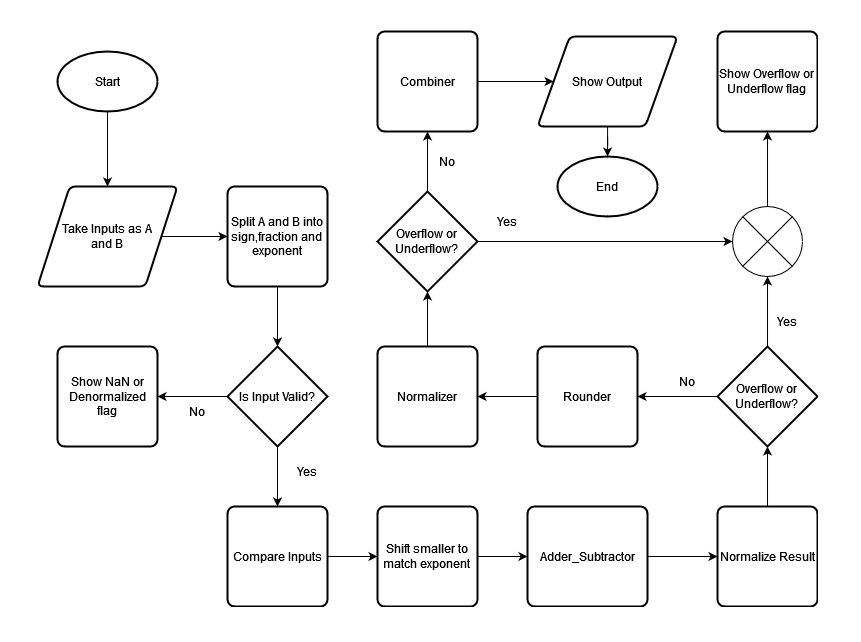
\includegraphics[width=0.8\textwidth]{images/flowchart.png}
	\caption{ Flowchart of the addition/subtraction algorithm }
	\label{fig:enter-label}
\end{figure}





\newpage



\section{\large{High-level block diagram of the architecture}}


\vspace{15mm}
\begin{figure}[H]
	\centering
	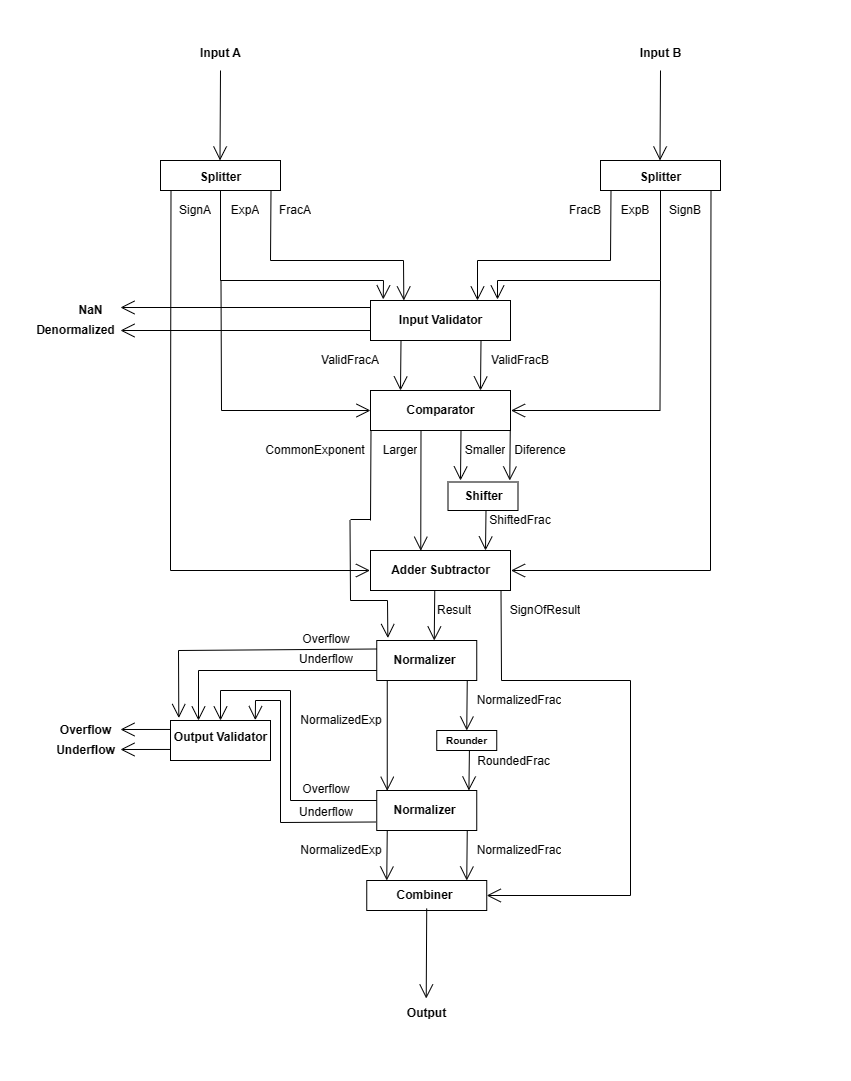
\includegraphics[width=0.8\textwidth]{images/fpa-block.png}
	\caption{ Flowchart of the addition/subtraction algorithm }
	\label{fig:enter-label}
\end{figure}


\newpage



% Muhit



\section{\large{Detailed Circuit Diagram of the Important Blocks}}
Some libraries and circuits were implemented to enhance and simplify the final circuit design.Those are :

\subsection{Multiplexer Circuits}
The modular circuits in this library are as follows 
\begin{itemize}

    \item 11 bit 2 to 1 Mux 
    \item 12 bit 2 to 1 Mux 
    \item 32 bit 2 to 1 Mux 

\end{itemize}
\begin{figure}[H]
    \centering
    \begin{subfigure}[b]{0.3\textwidth}
        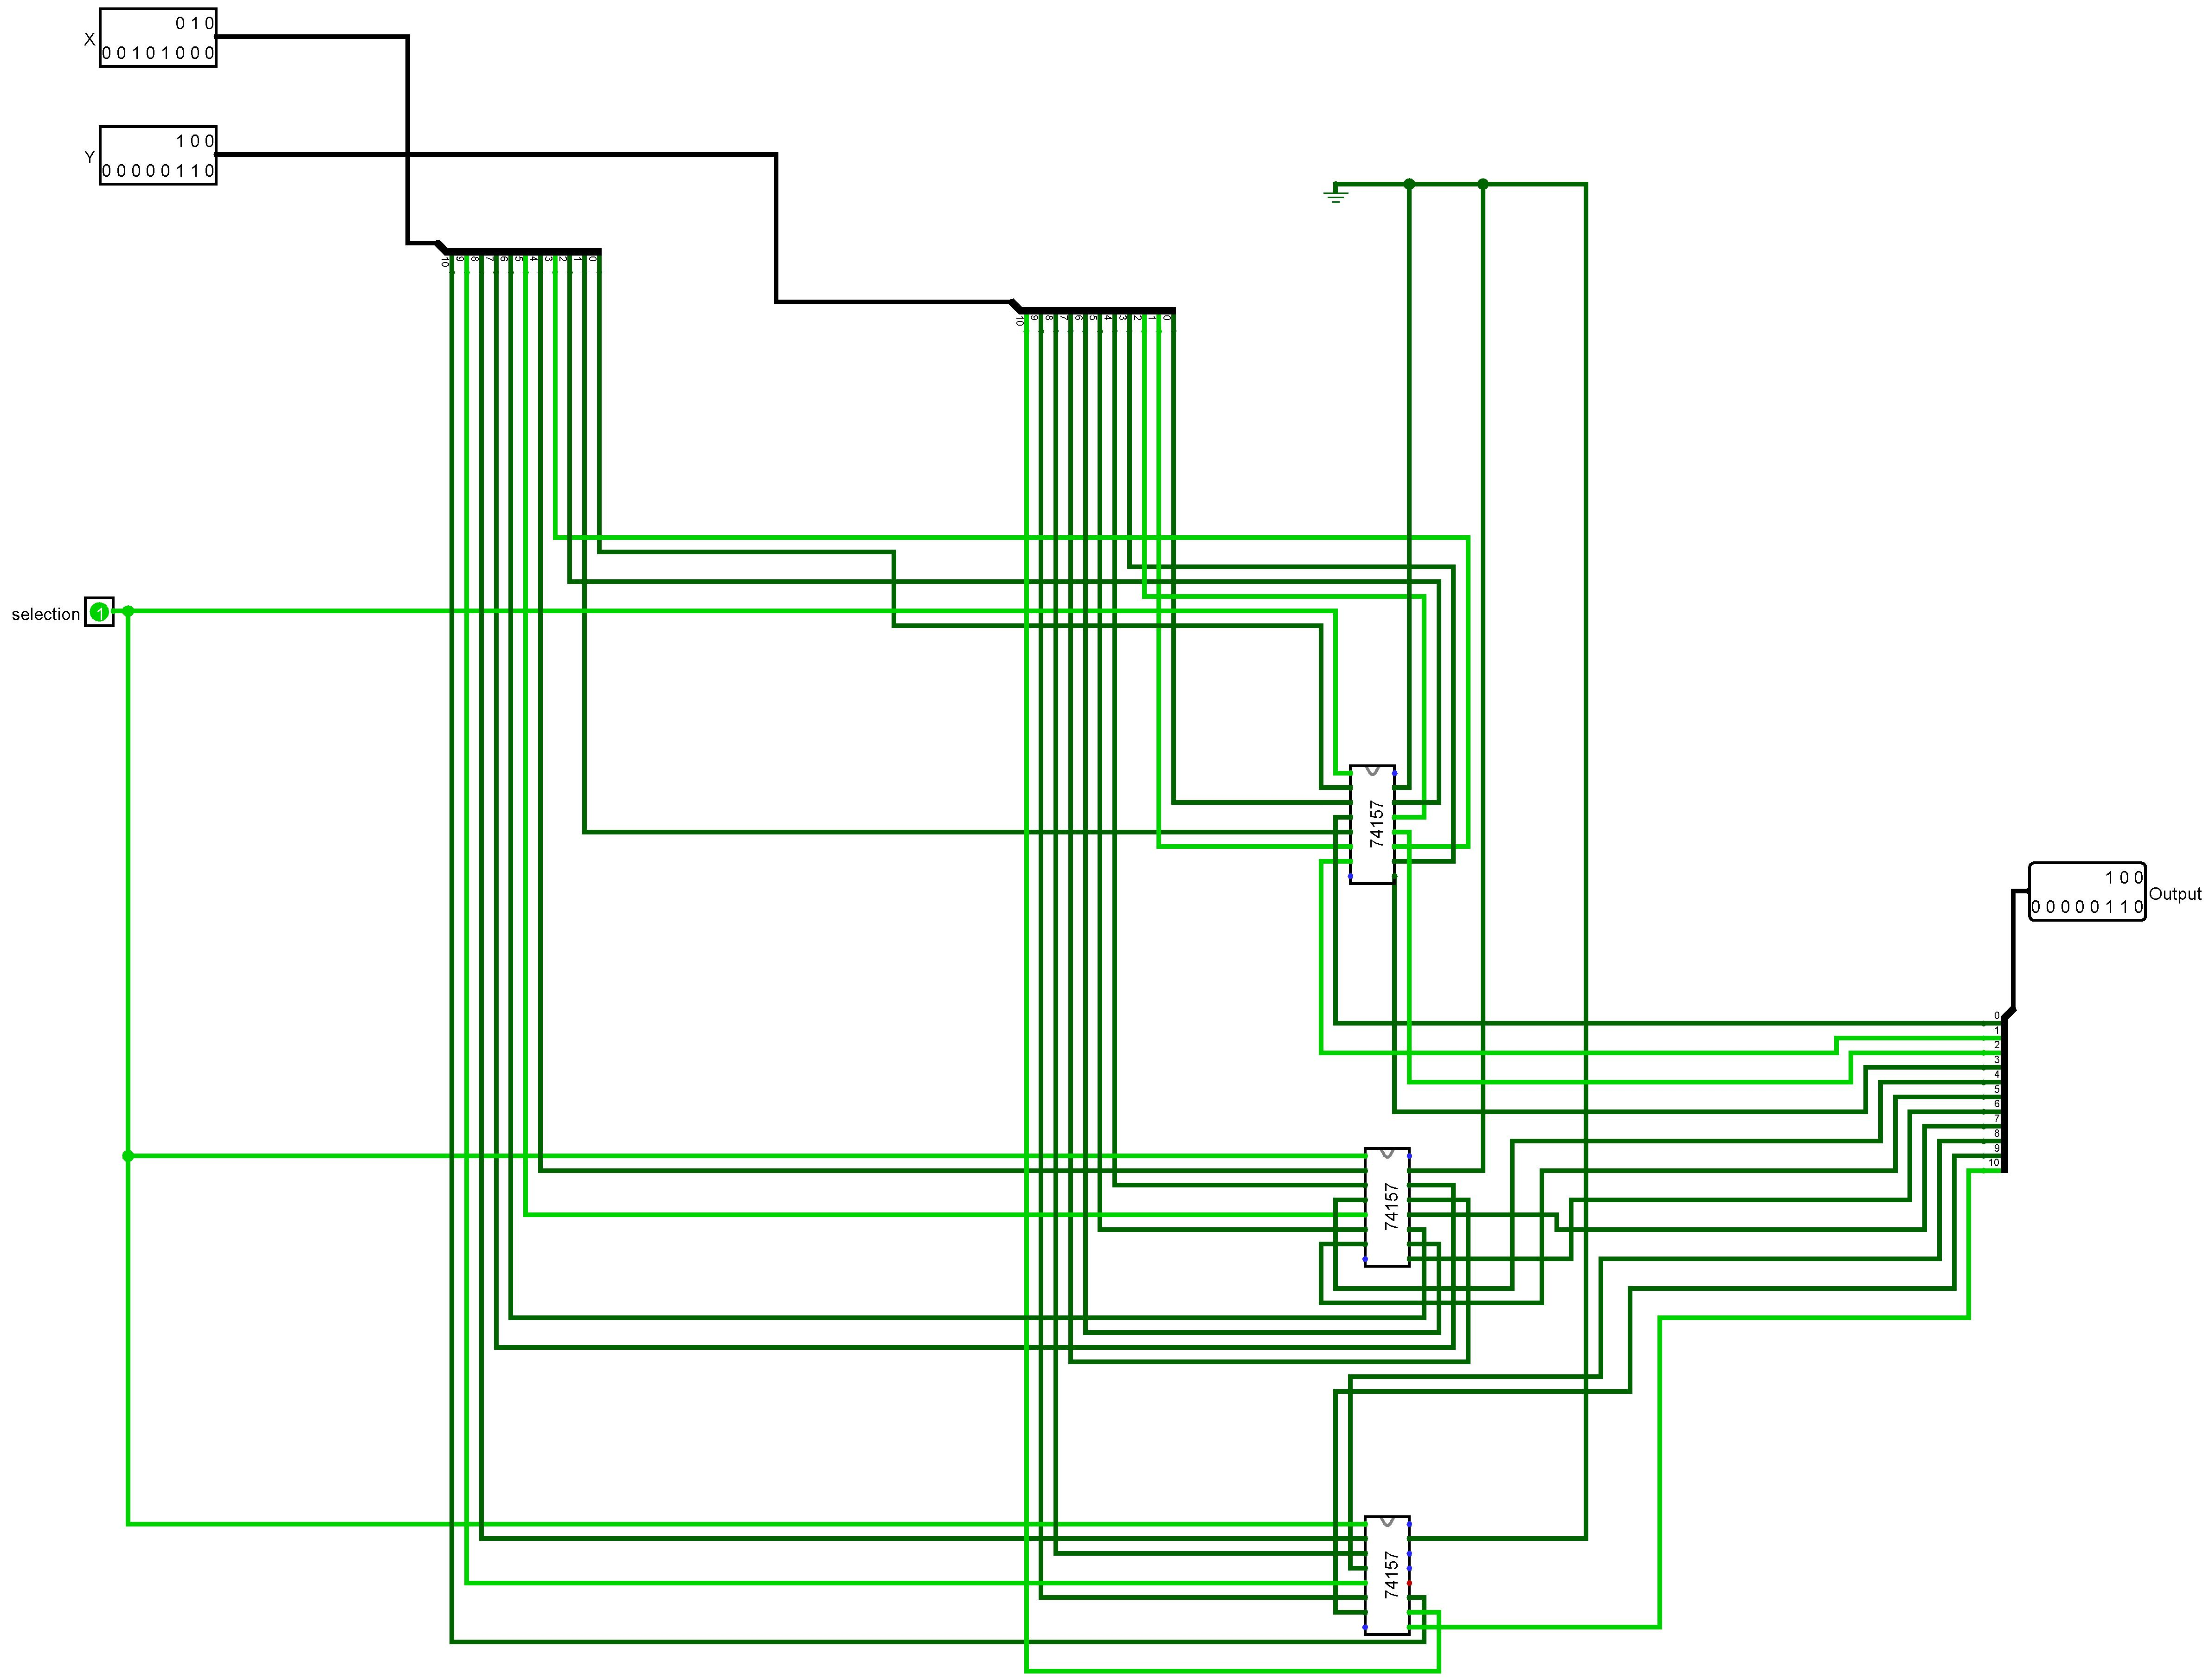
\includegraphics[width=\textwidth]{images/MUX_11_bit.jpg}
        \caption{11 bit $2\times1$ MUX}
        \label{fig:11b2x1mux}
    \end{subfigure}
    \begin{subfigure}[b]{0.3\textwidth}
        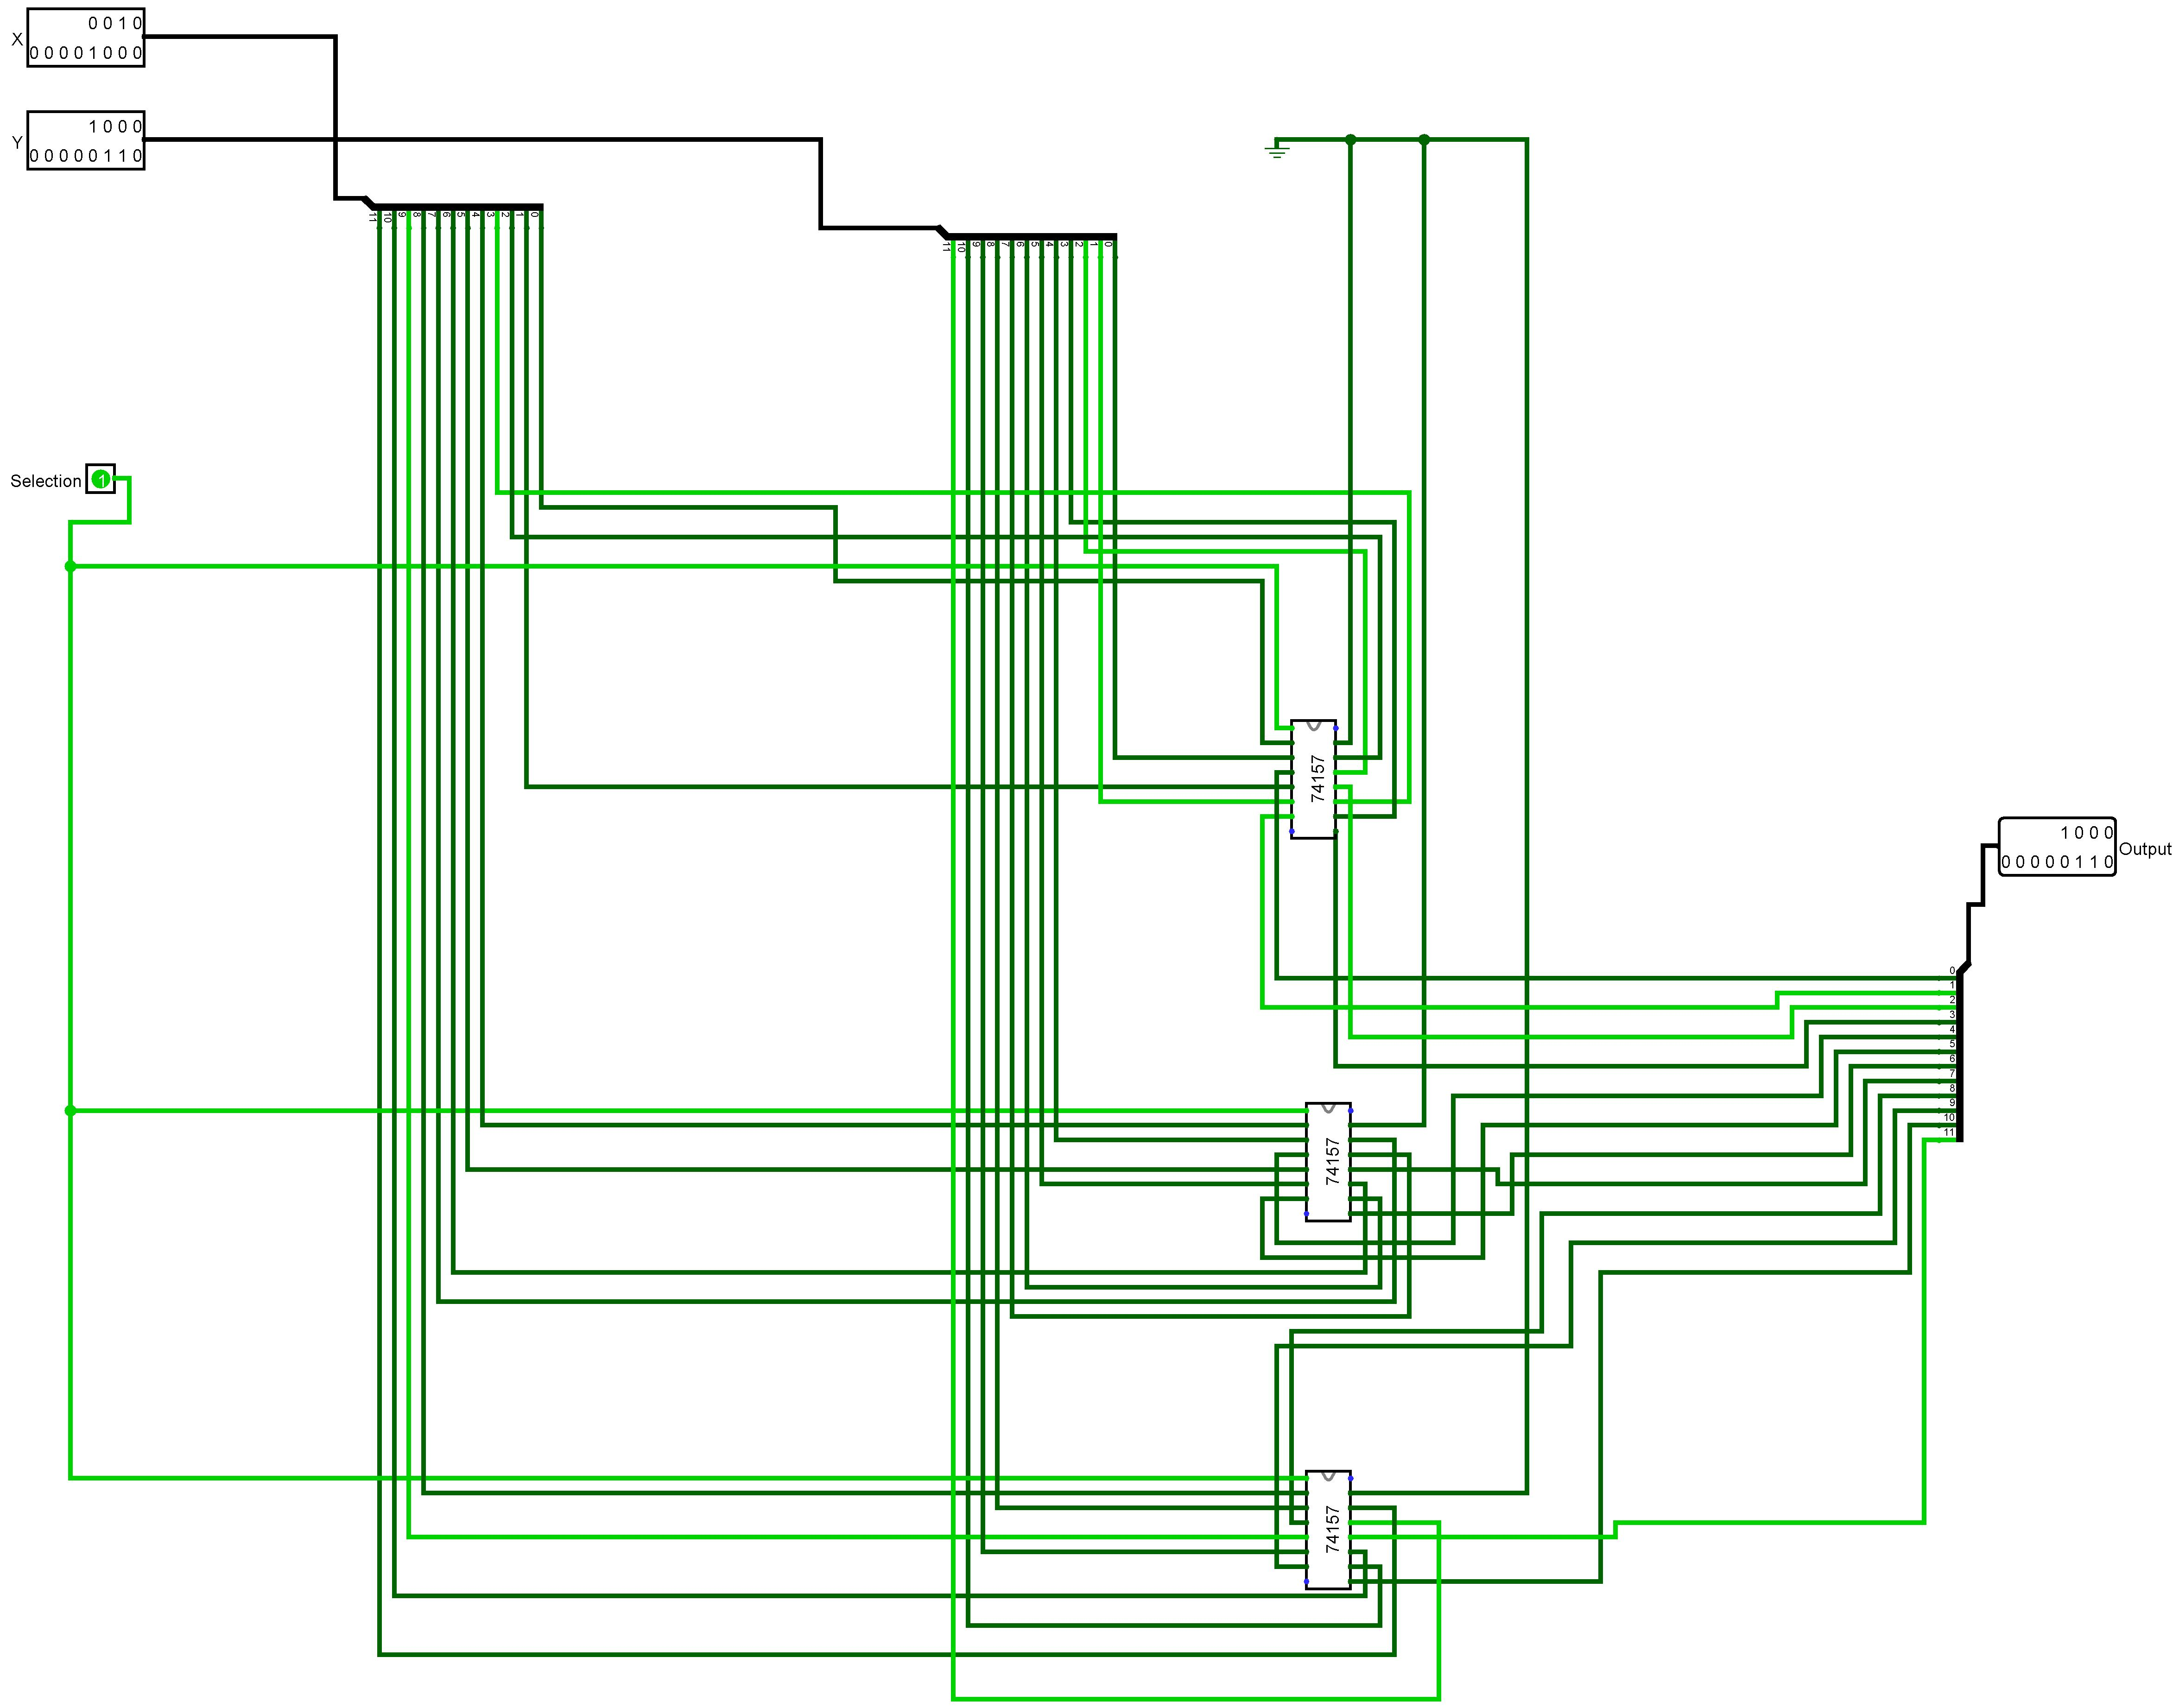
\includegraphics[width=\textwidth]{images/MUX_12_bit.jpg}
        \caption{12 bit $2\times1$ MUX}
        \label{fig:12b2x1mux}
    \end{subfigure}
     \newline
     \newline
    \begin{subfigure}[b]{0.4\textwidth}
        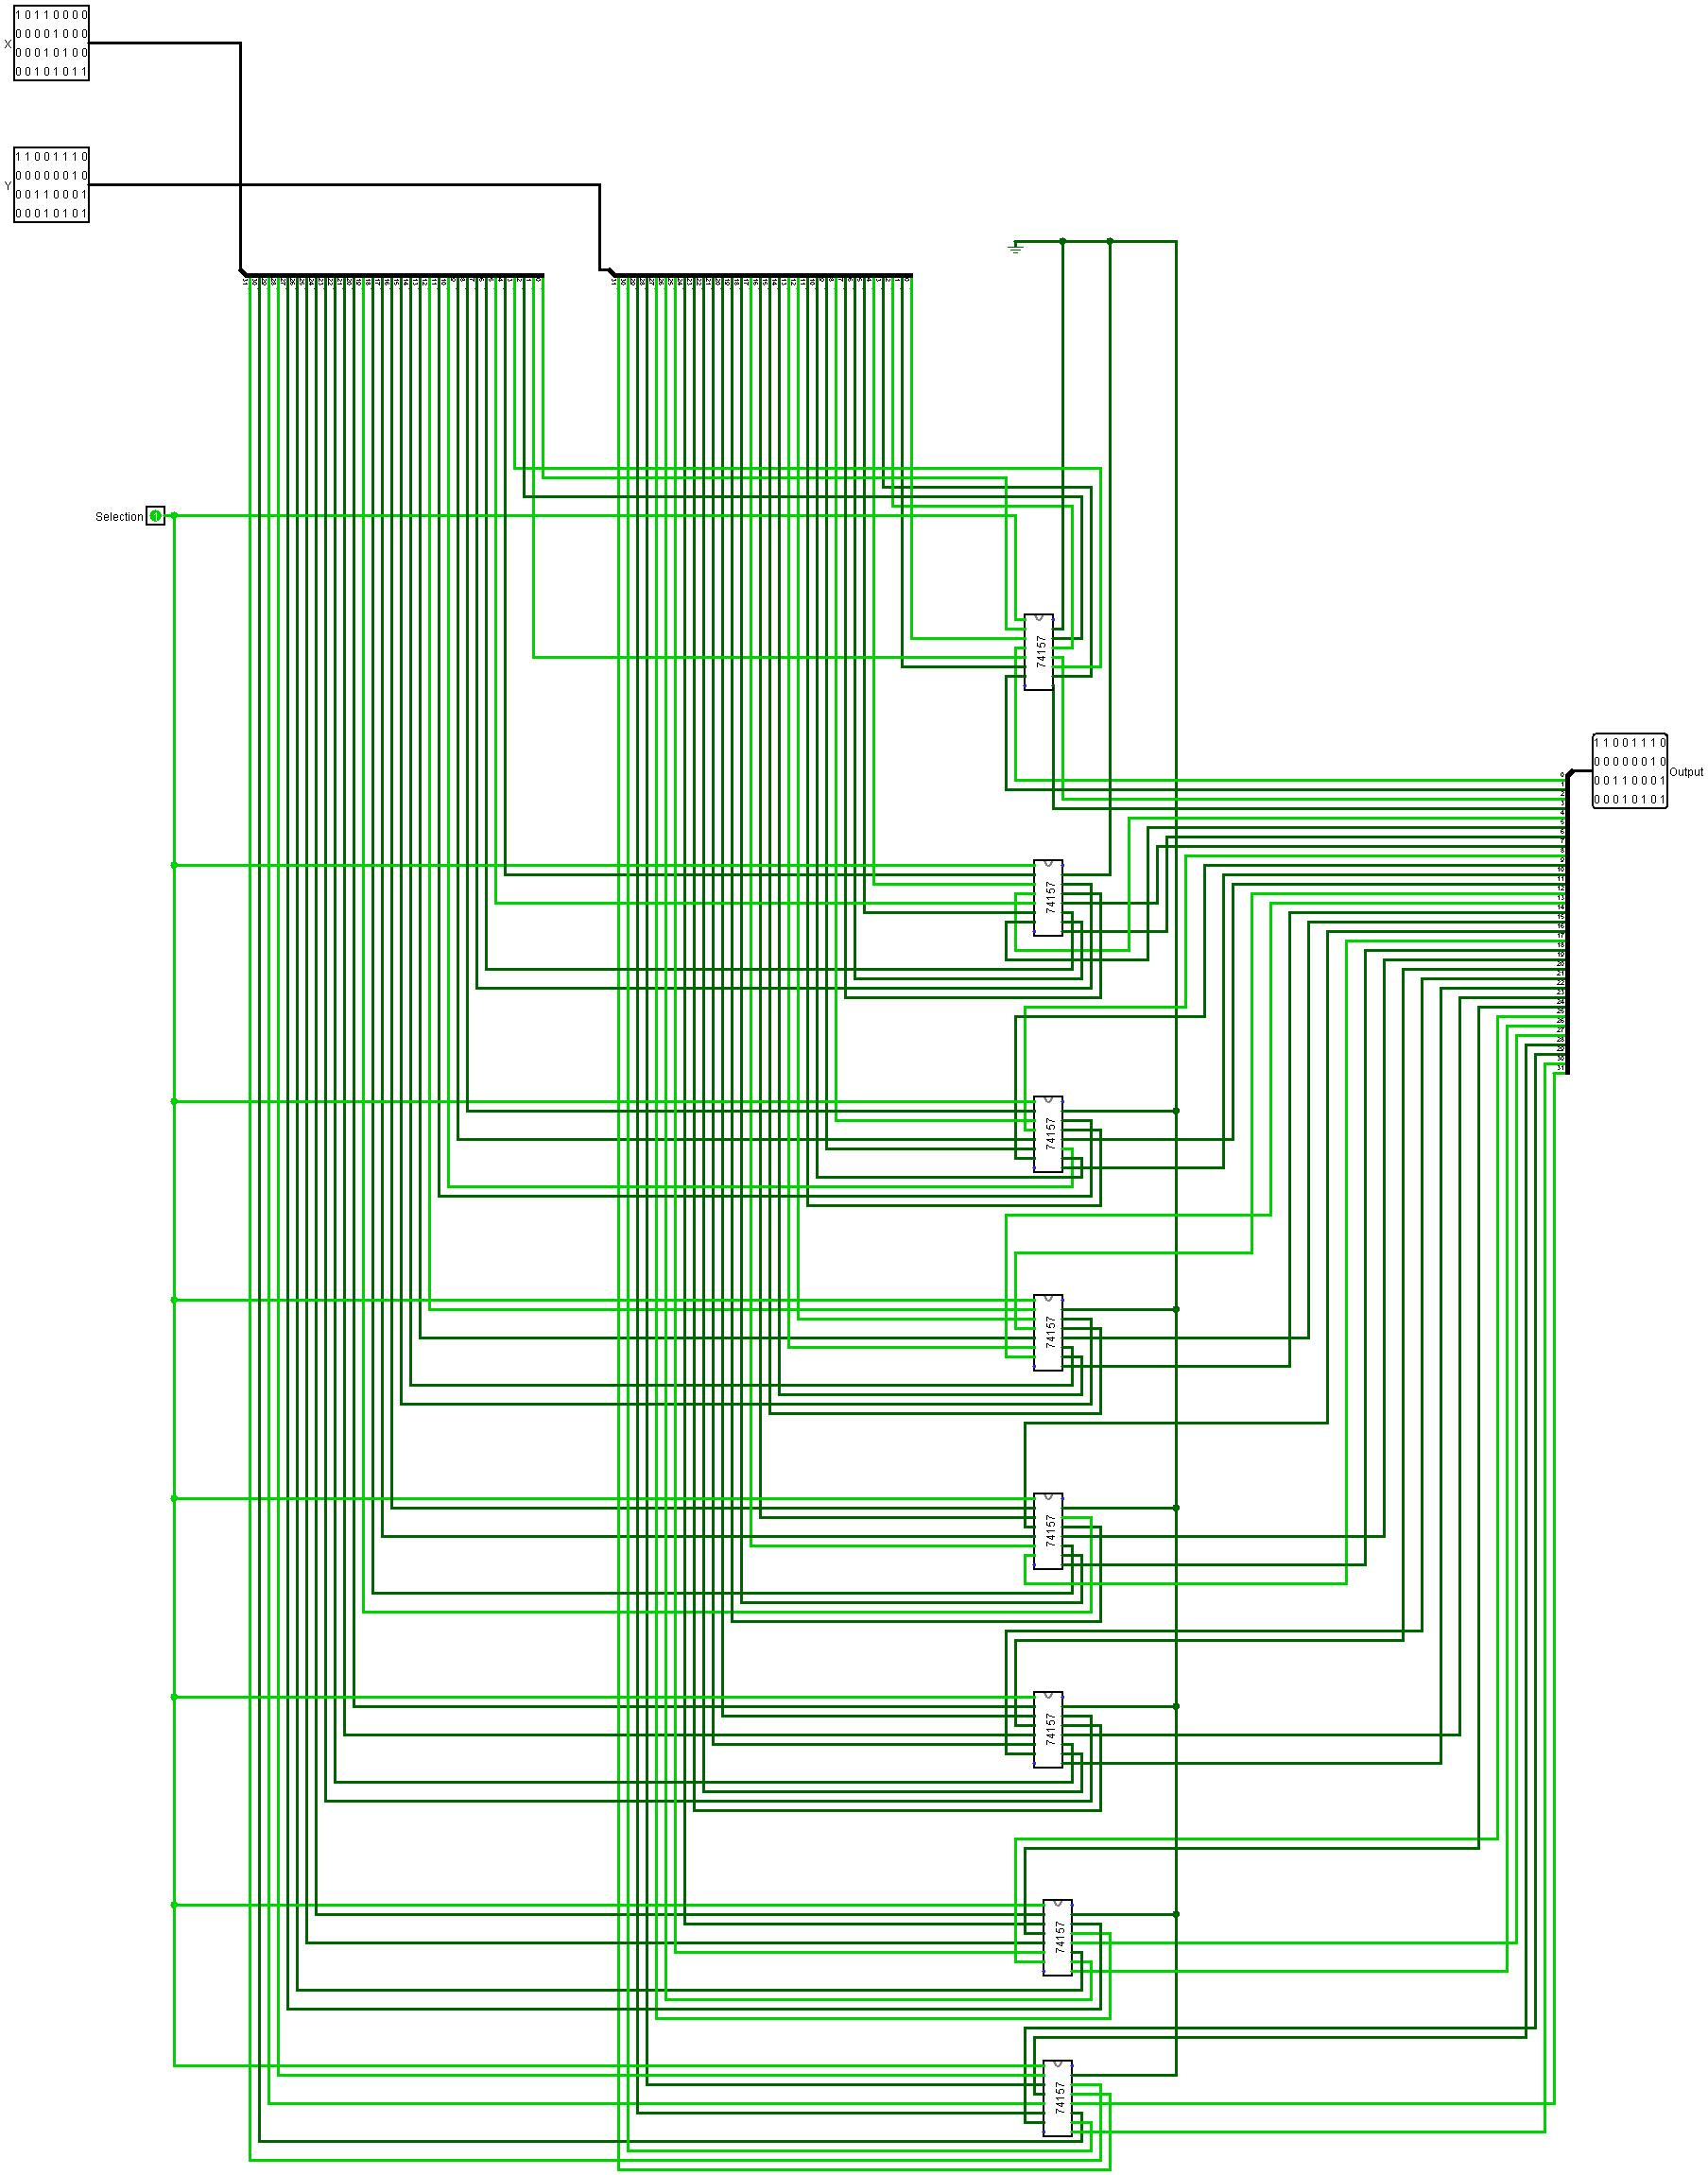
\includegraphics[width=\textwidth]{images/MUX_32_bit.jpg}
        \caption{32 bit $2\times1$ MUX}
        \label{fig:32b2x1}
    \end{subfigure}

    \caption{Multiplexer Circuits}\label{fig:mux}
\end{figure}

\newpage

\subsection{Comparator Circuits}
An comparator library was constructed to compare the exponenets . This library contains 2 circuits i.e. an 11 bit magnitude comparator and a comparator for small fractions.
\begin{figure}[H]
    \centering
    \begin{subfigure}{\textwidth}
    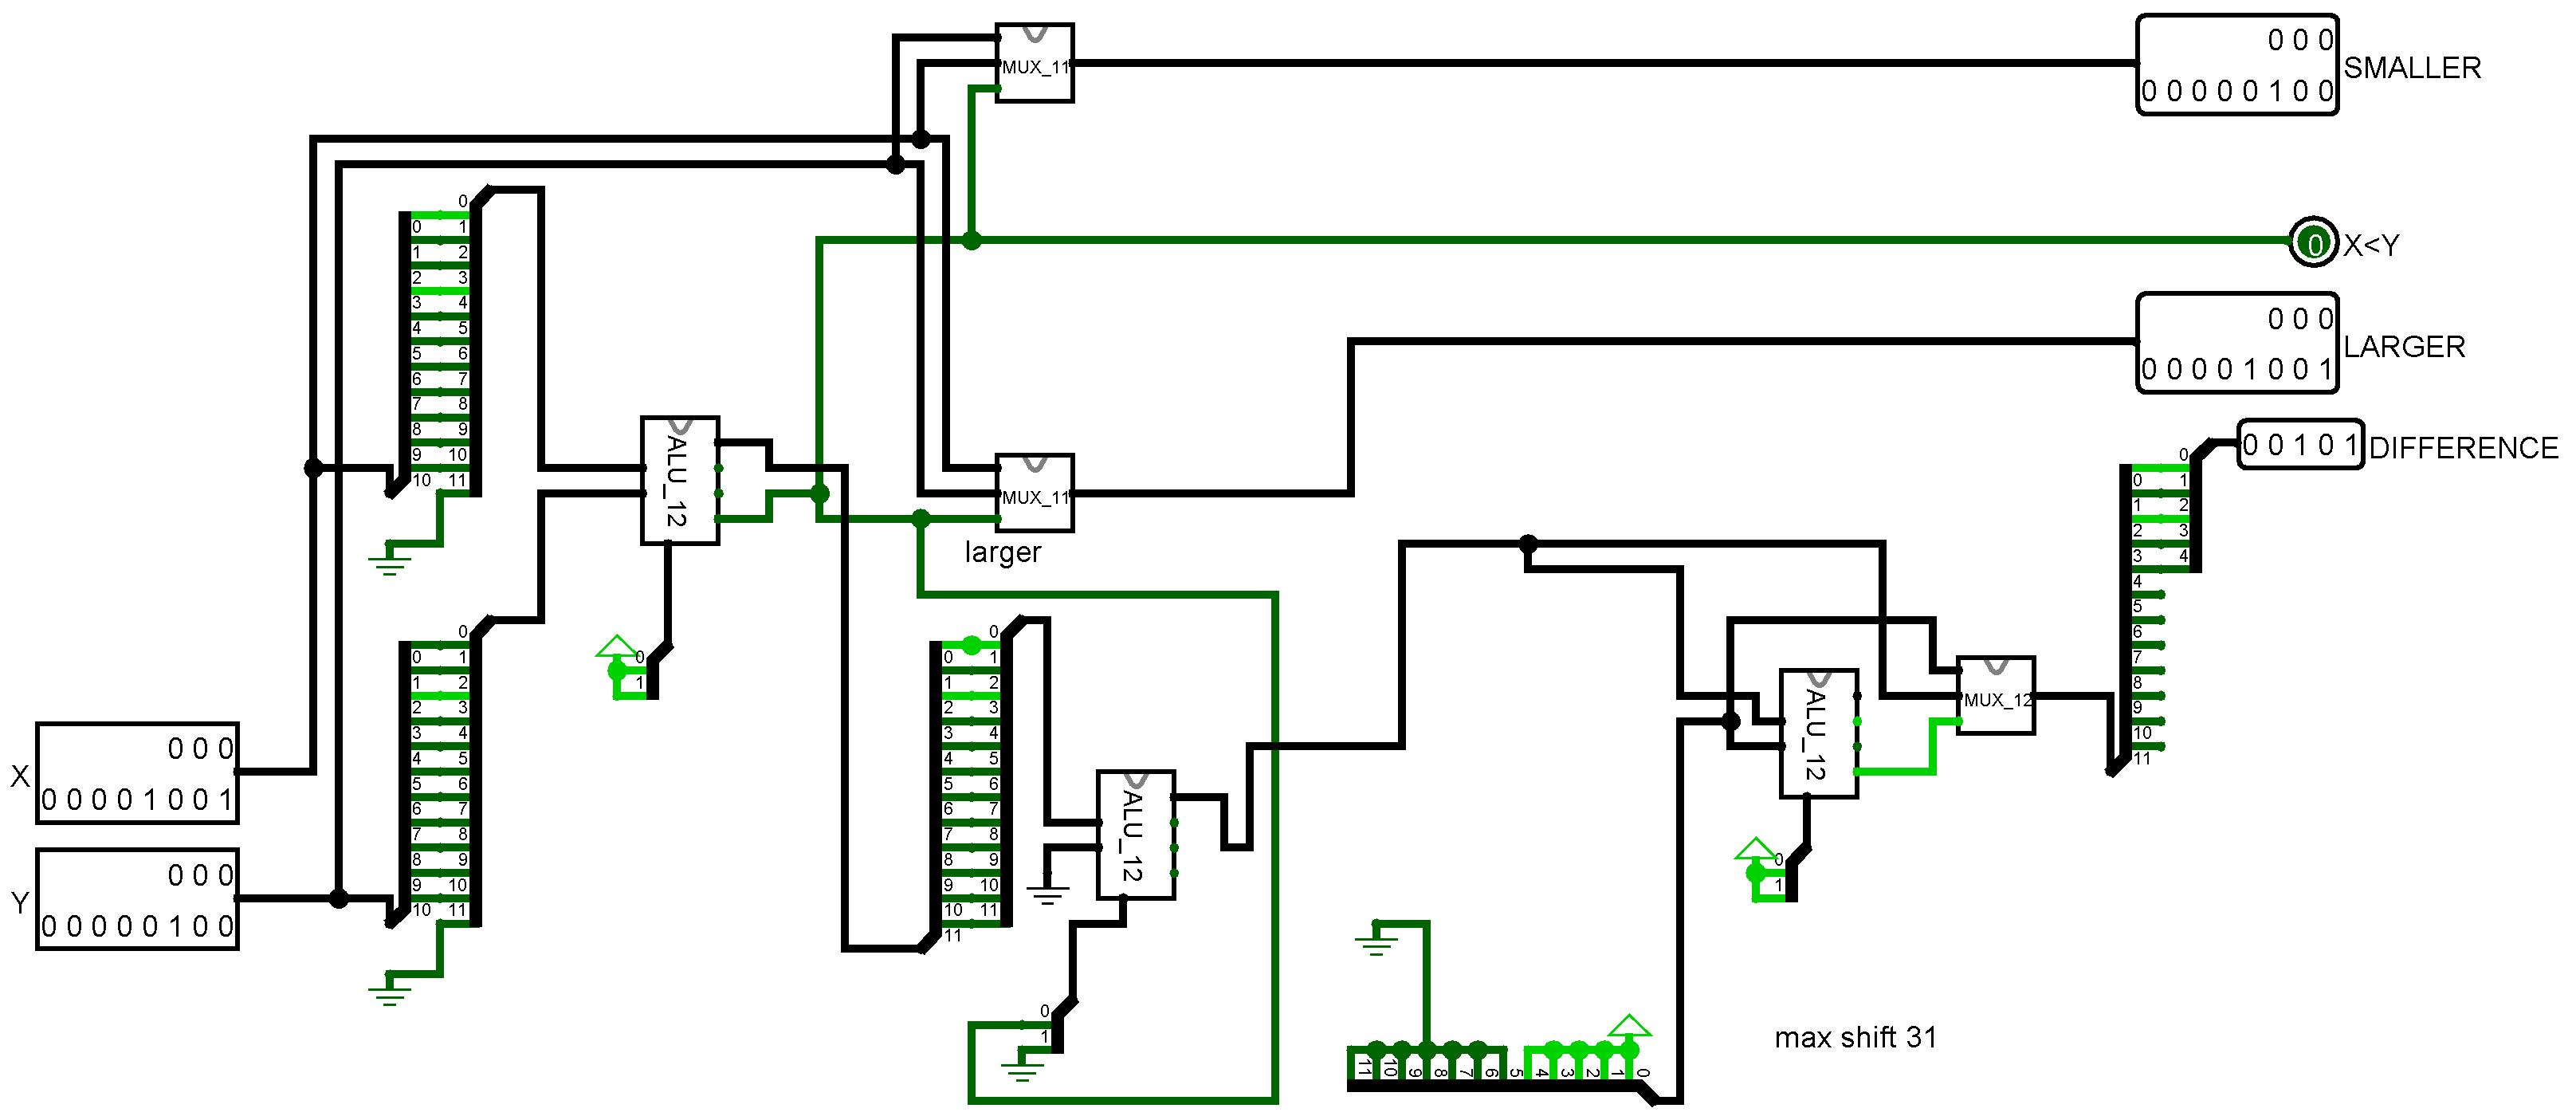
\includegraphics[width=\textwidth]
        {images/Comparator_11_bit.jpg}
        \label{fig:11bitmagcomp}
    \caption{11 Bit Magnitude Comparator}
        
    \end{subfigure}
    \begin{subfigure}{\textwidth}
    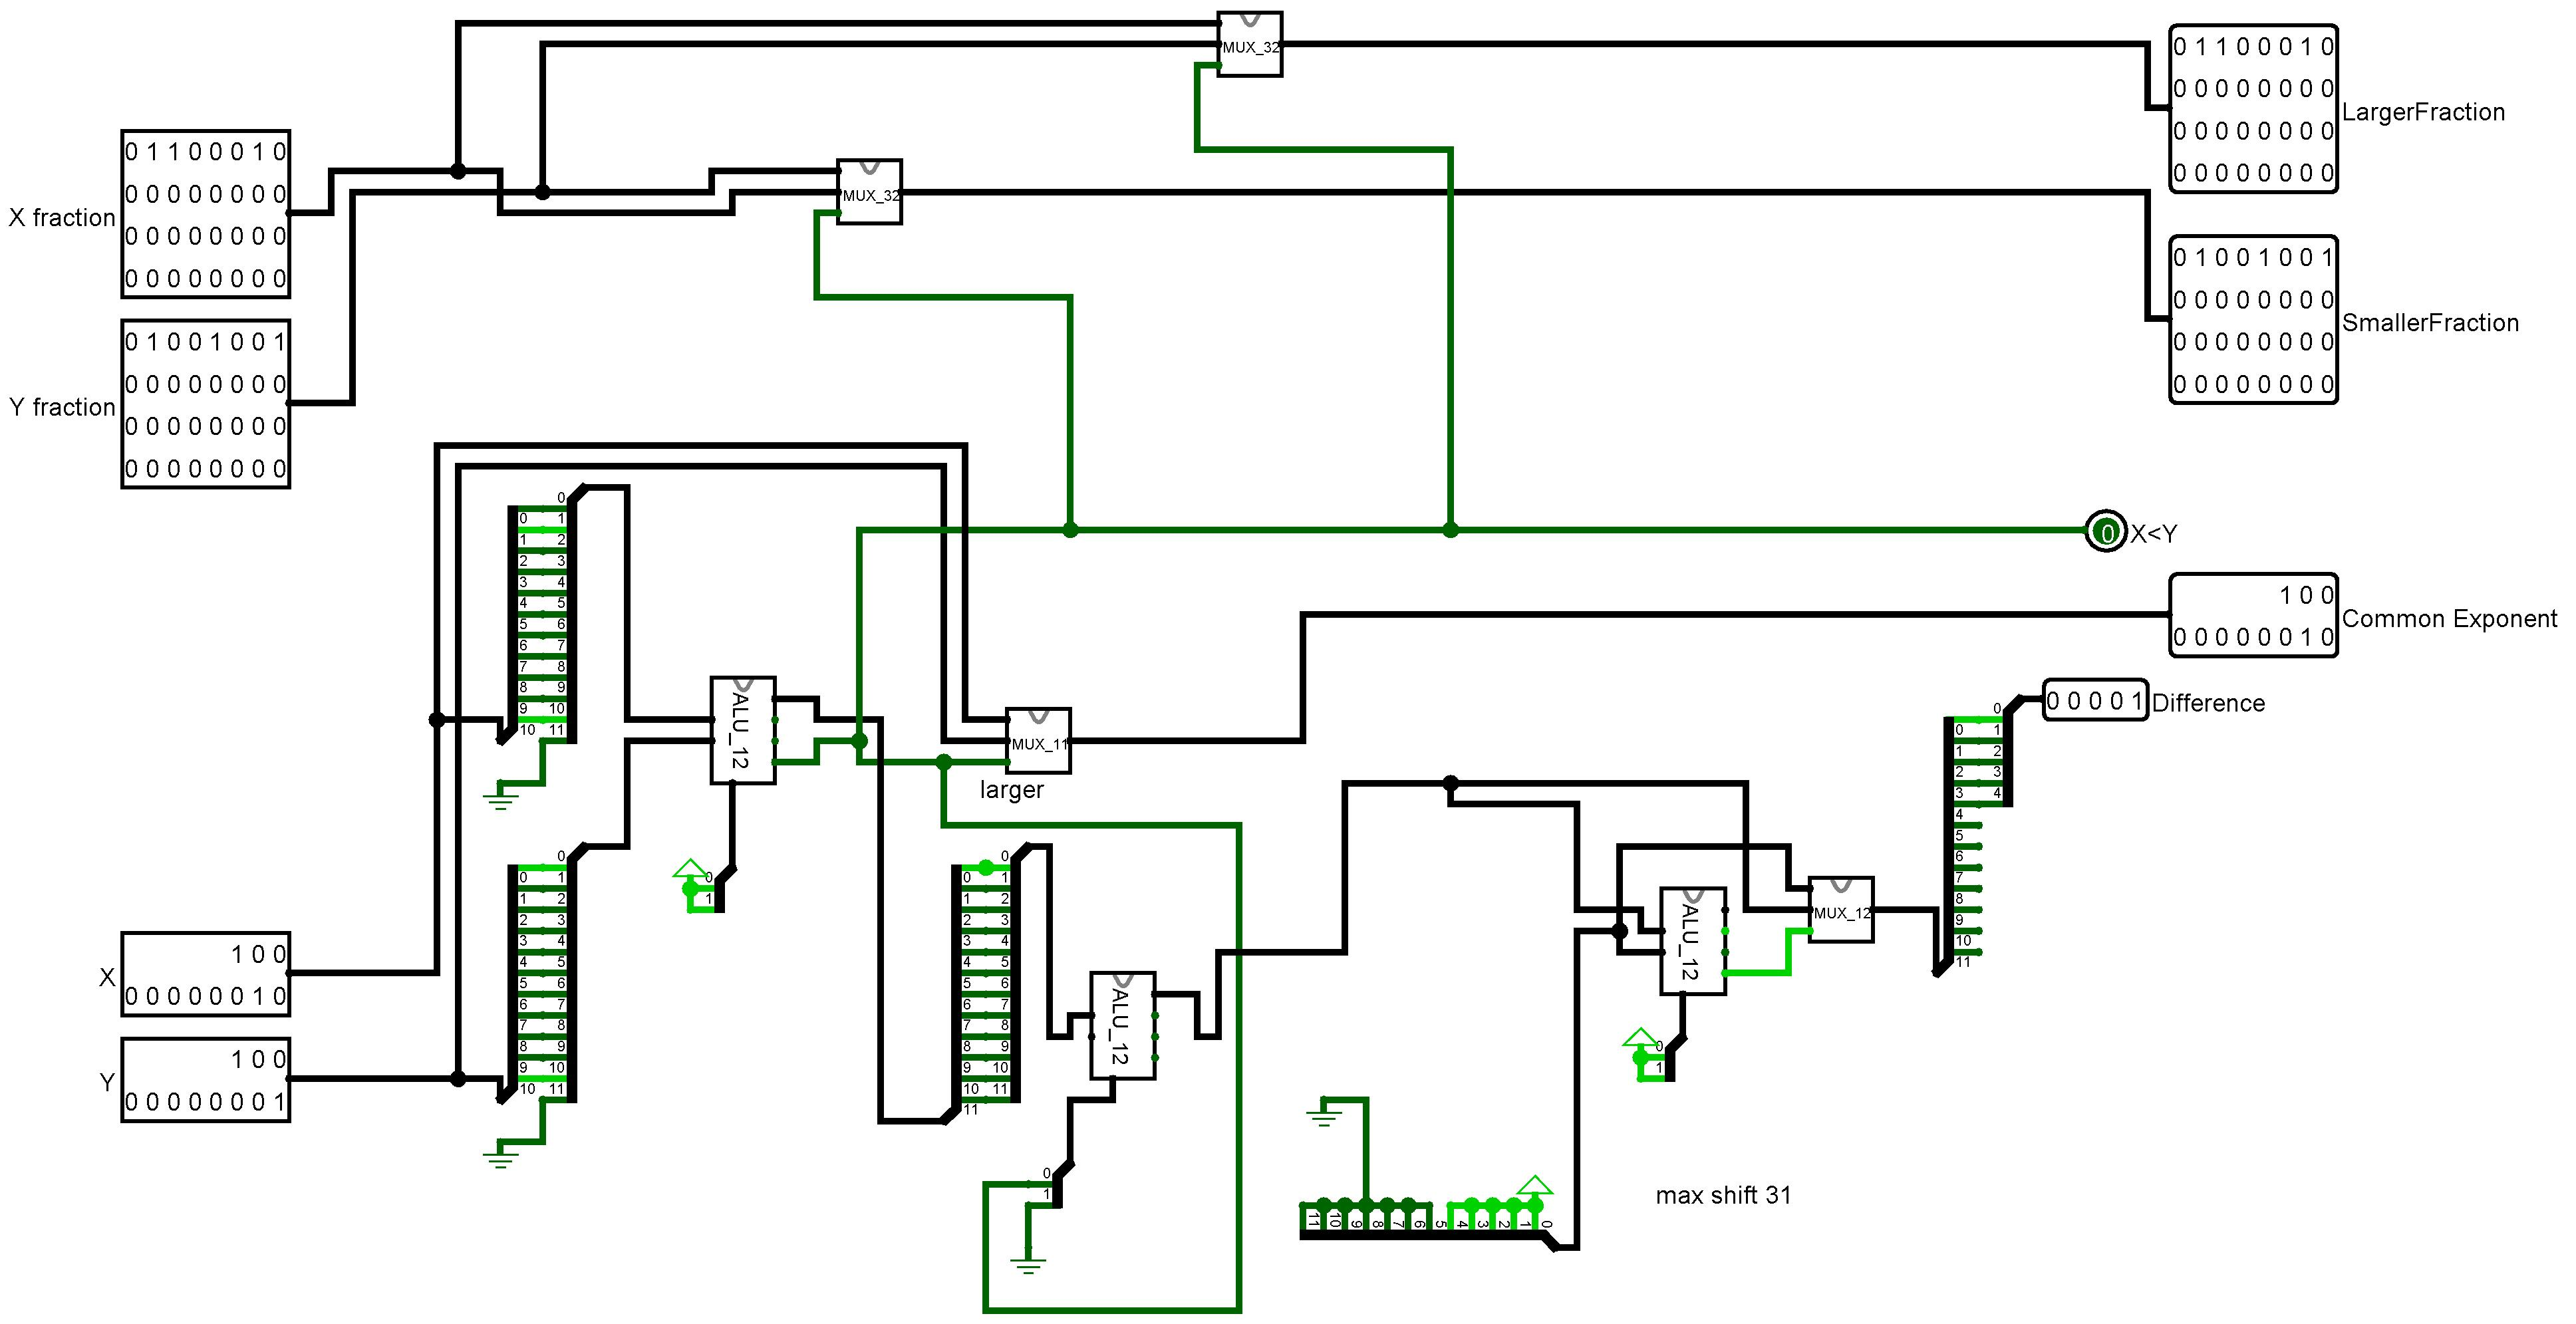
\includegraphics[width=\textwidth]
        {images/Comparator_With_Smaller_Fraction.jpg}
        \label{fig:smfracmagcomp}
    \caption{Smaller Fractions Magnitude Comparator}
        
    \end{subfigure}
    \label{fig:magcomps}
    \caption{Magnitude Comparators}
        
\end{figure}
\newpage
\subsection{Adder-Subtractor Circuit}
A 32 bit adder-subtractor circuit was implemented to add or subtract 2 signed numbers
\begin{figure}[H]
    \centering
        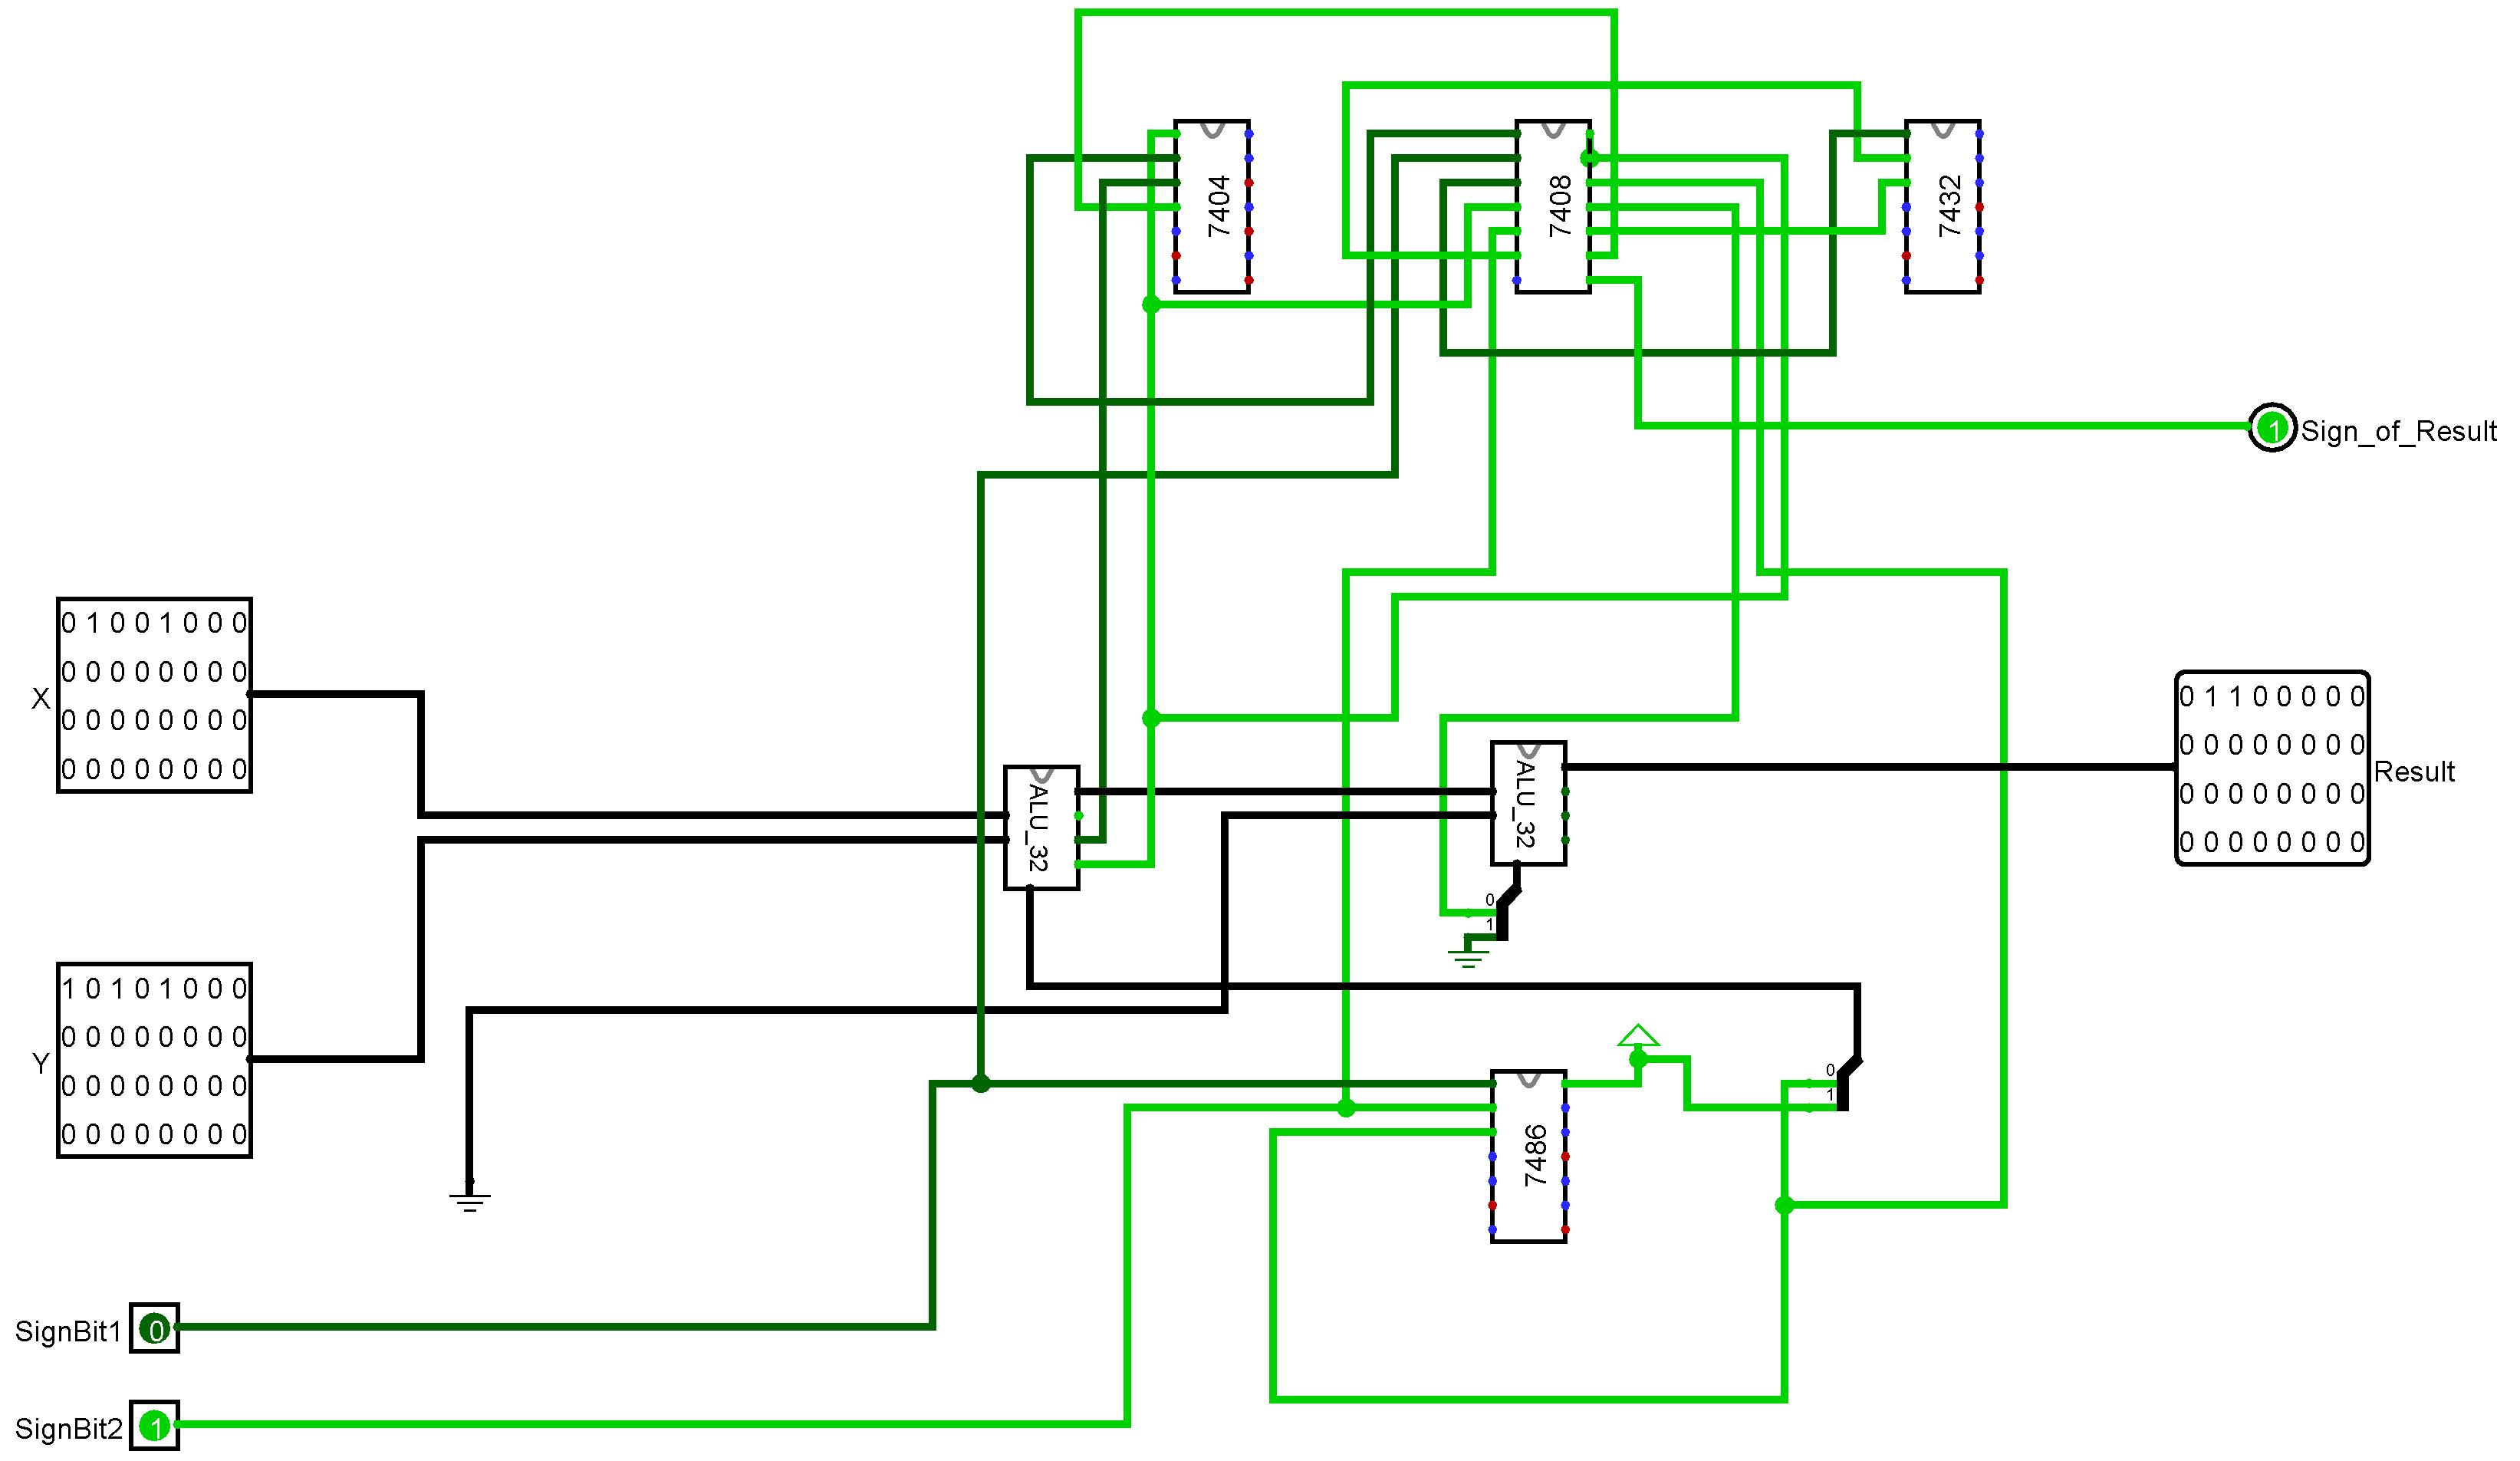
\includegraphics[width=\textwidth]{images/Adder_Subtractor.jpg}
        \caption{32 bit Adder$-$Subtractor}
        \label{fig:32bitaddsub}
\end{figure}

\newpage
\subsection{Encoder Circuits}
To normalize a number, we need to locate the first set bit starting from MSB. 3 priority encoders was used for this purpose. Those are :
\begin{itemize}
    \item 8 to 3 priority encoder 
    \item 16 to 4 priority encoder 
    \item 32 to 5 priority encoder 
\end{itemize}
\begin{figure}[H]
    \centering
    \begin{subfigure}[b]{0.45\textwidth}
        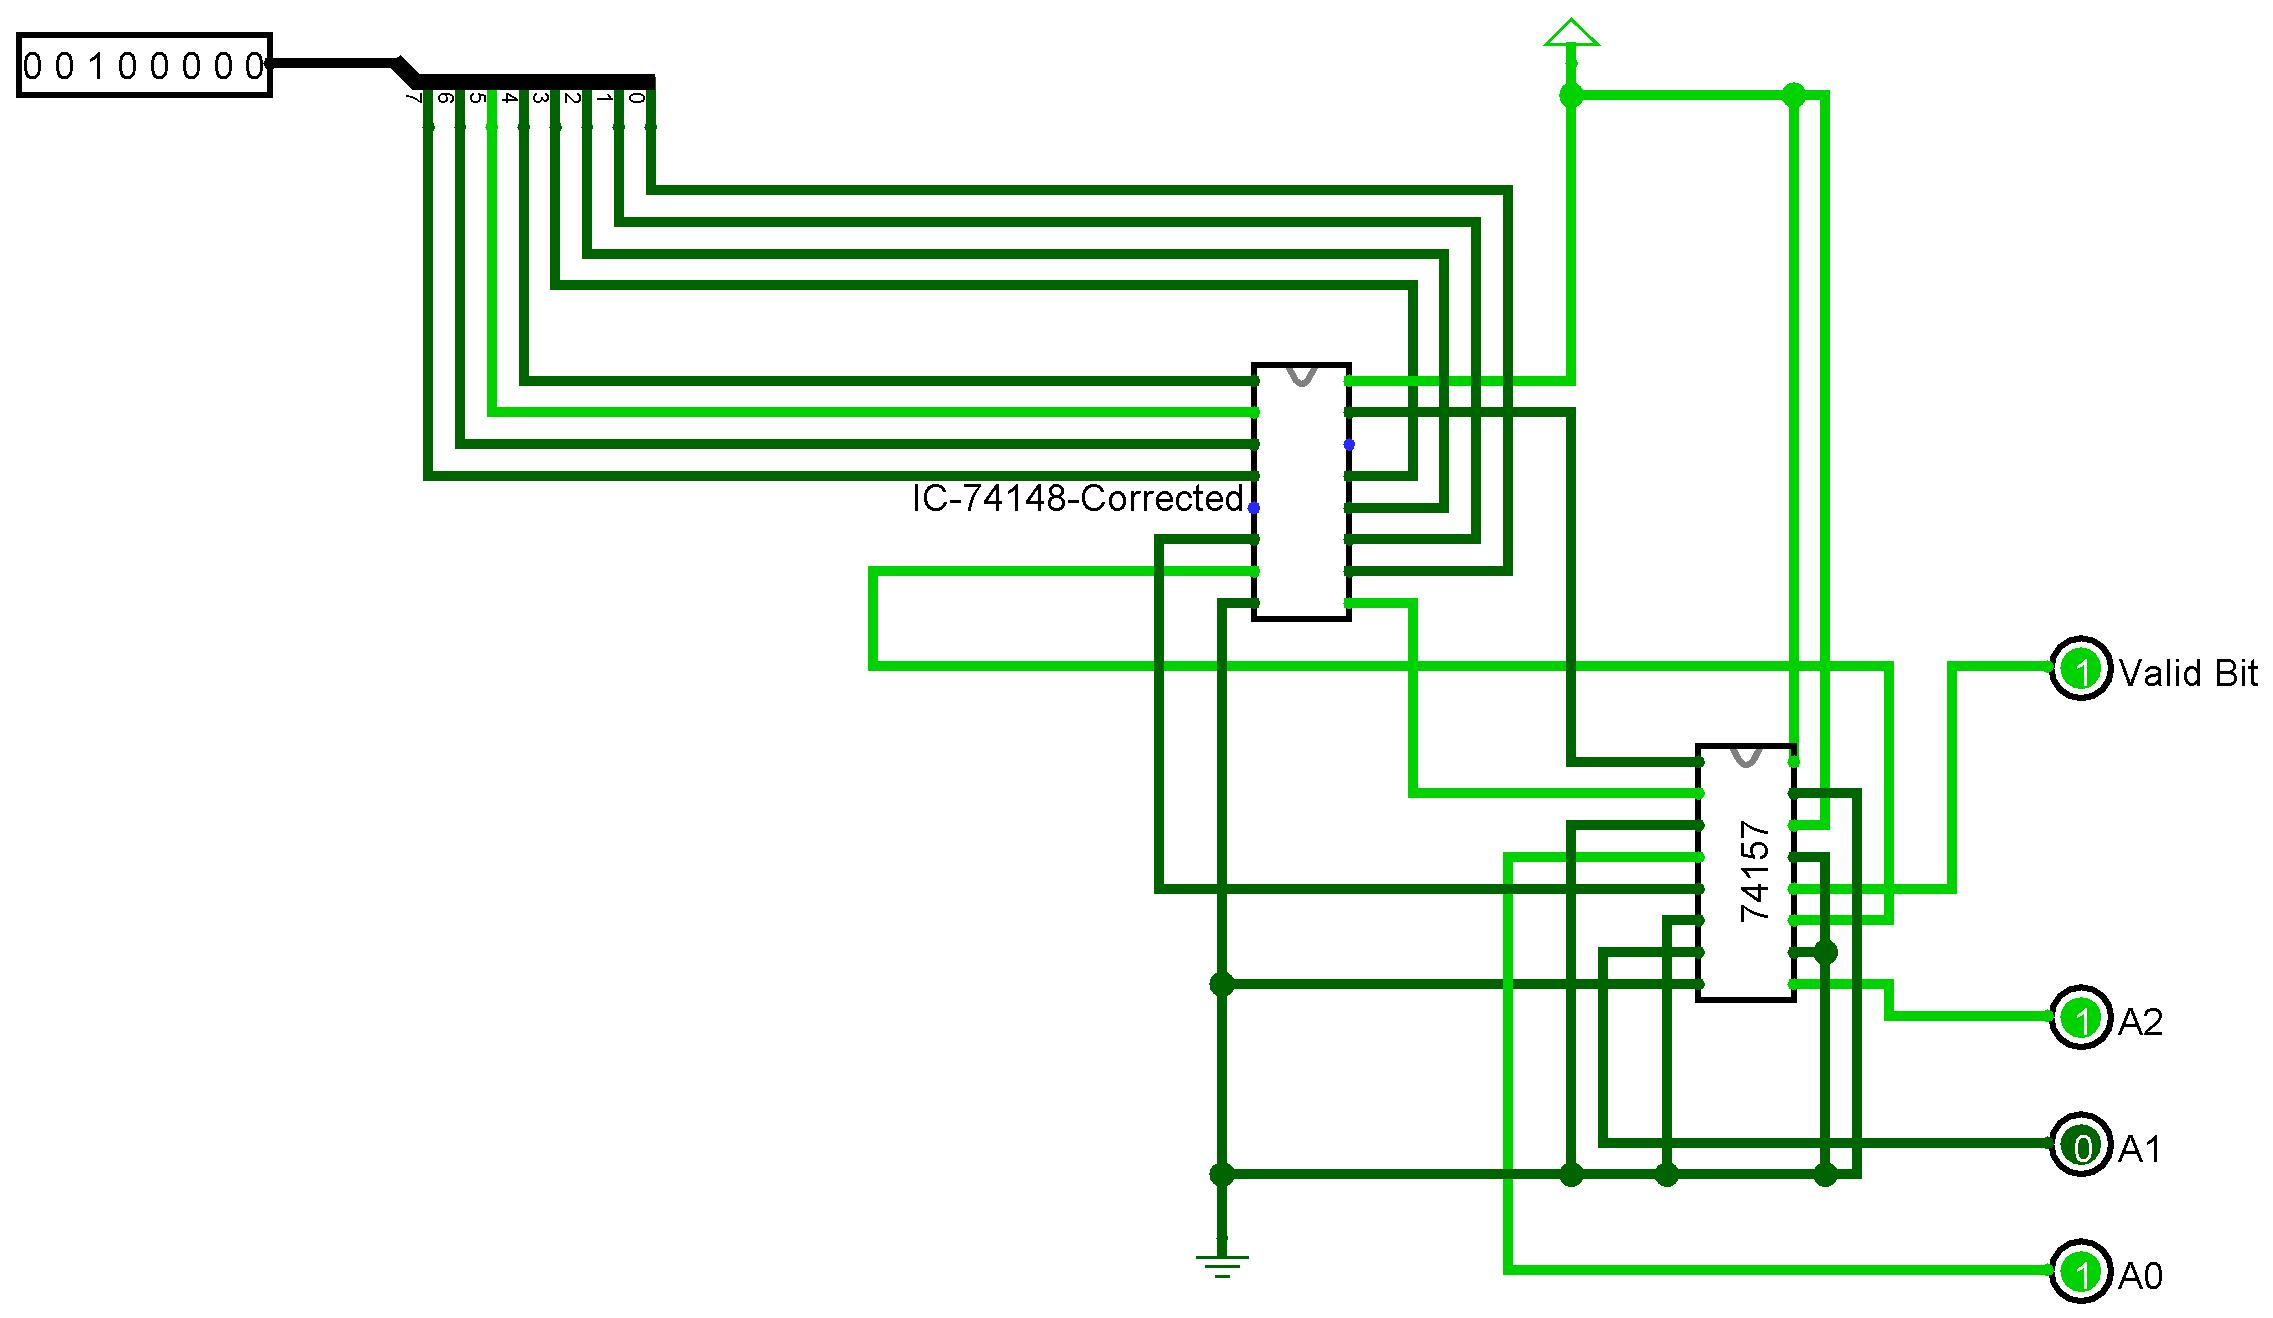
\includegraphics[width=\textwidth]{images/PE_8x3.jpg}
        \caption{8$\times$3 Priority Encoder}
        \label{fig:8x3prioenc}
    \end{subfigure}
    \begin{subfigure}[b]{0.45\textwidth}
        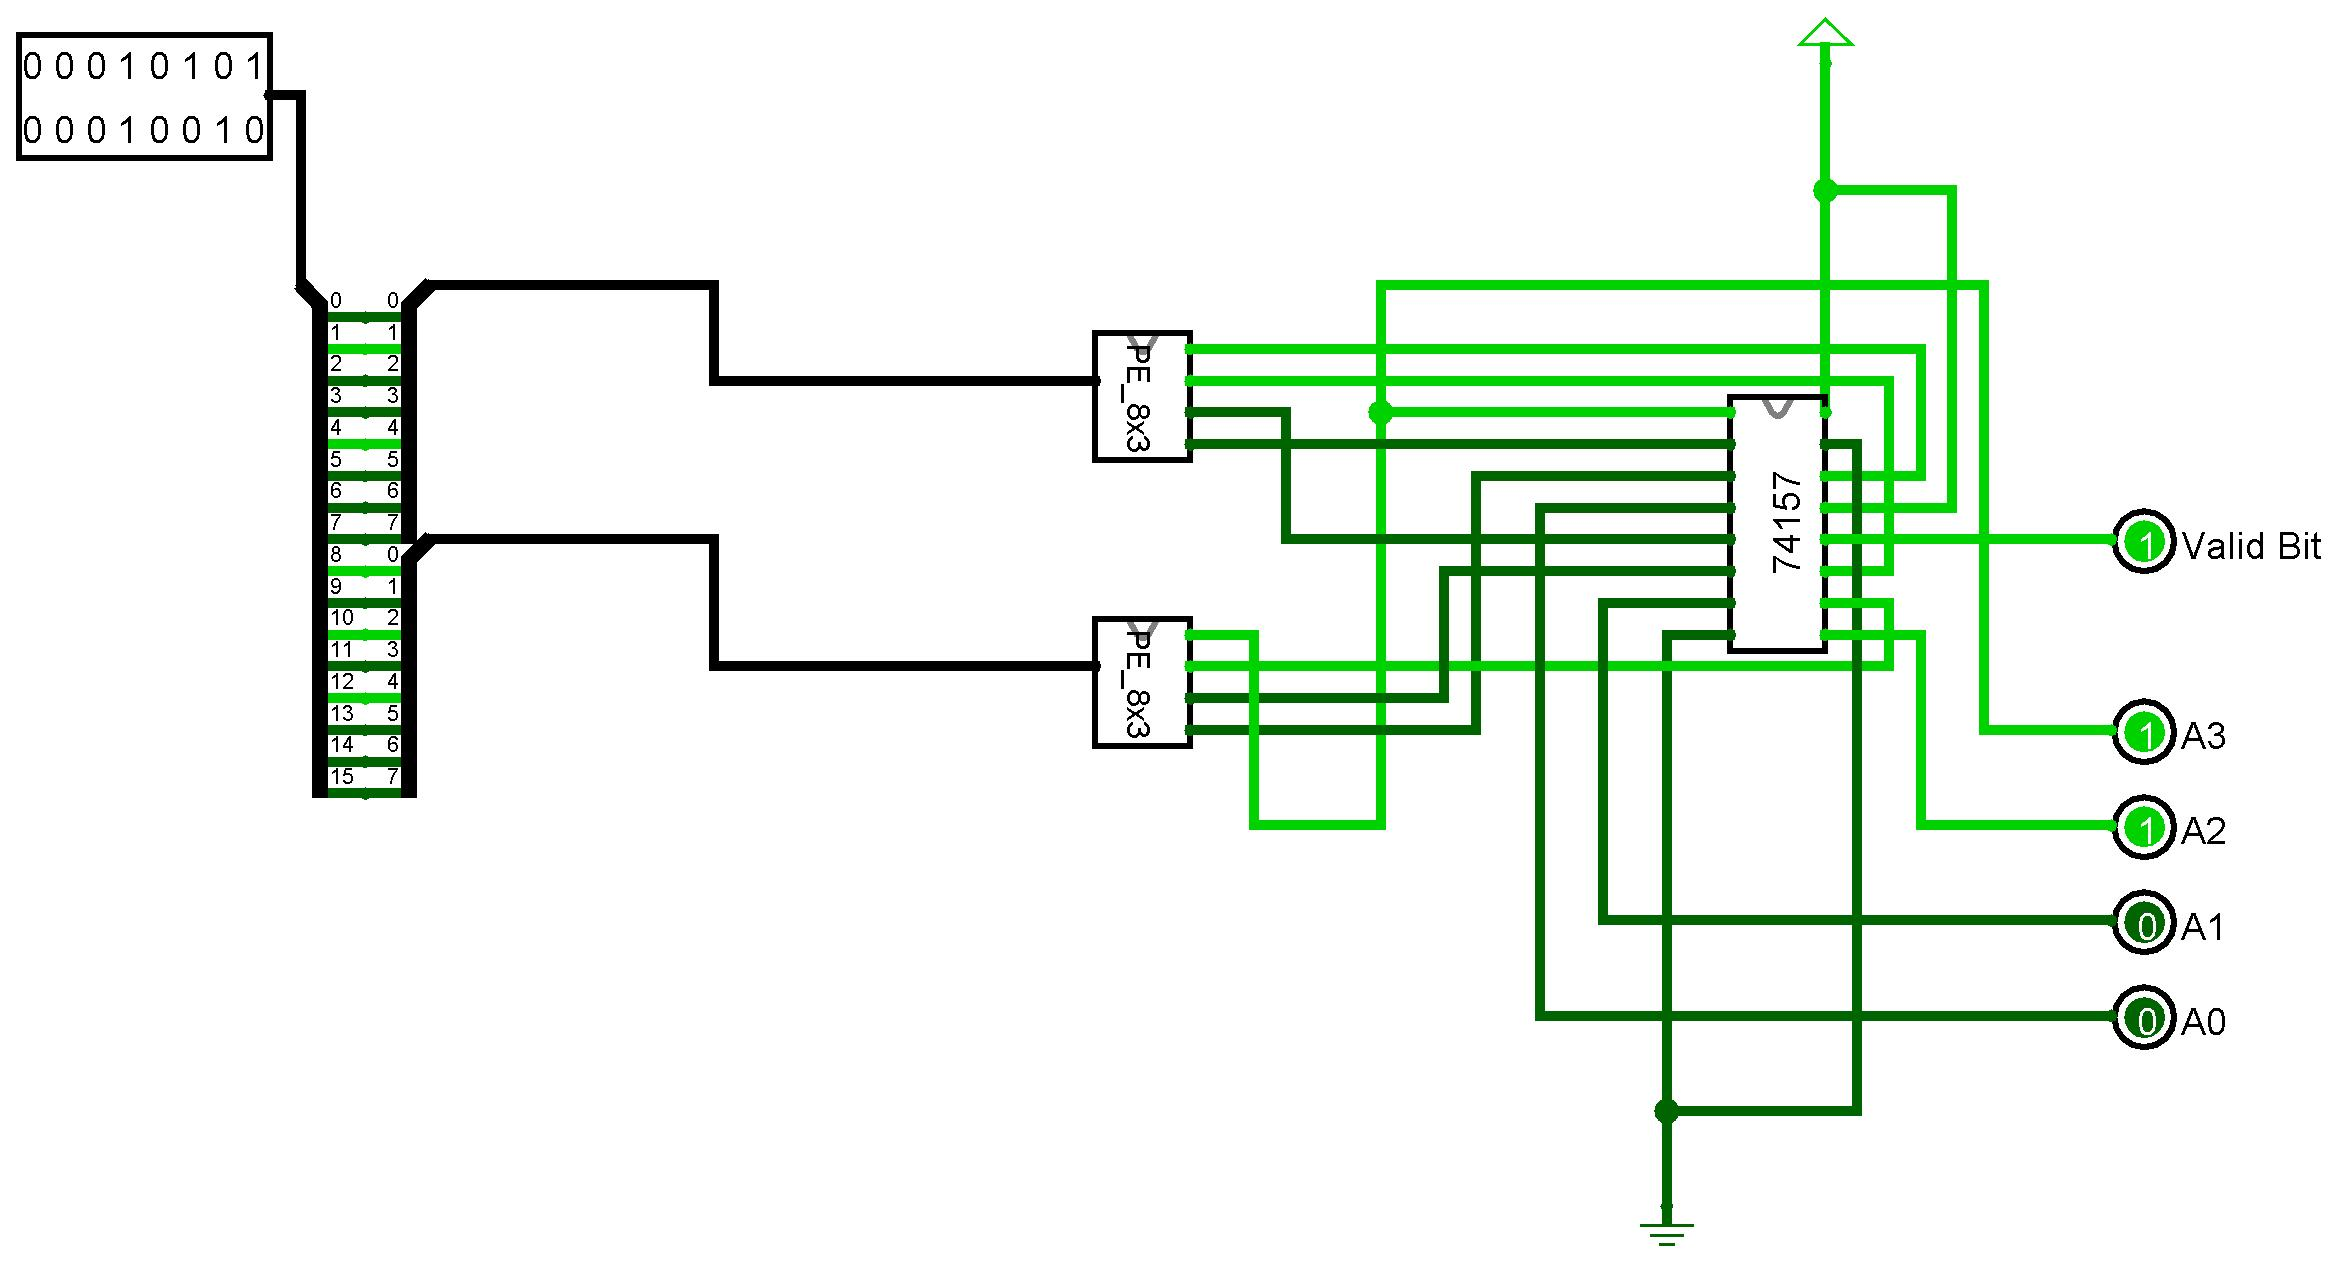
\includegraphics[width=\textwidth]{images/PE_16x4.jpg}
        \caption{16$\times$4 Priority Encoder}
        \label{fig:16x4prioenc}
    \end{subfigure}
    \newline
    \newline
    \begin{subfigure}[b]{0.9\textwidth}
        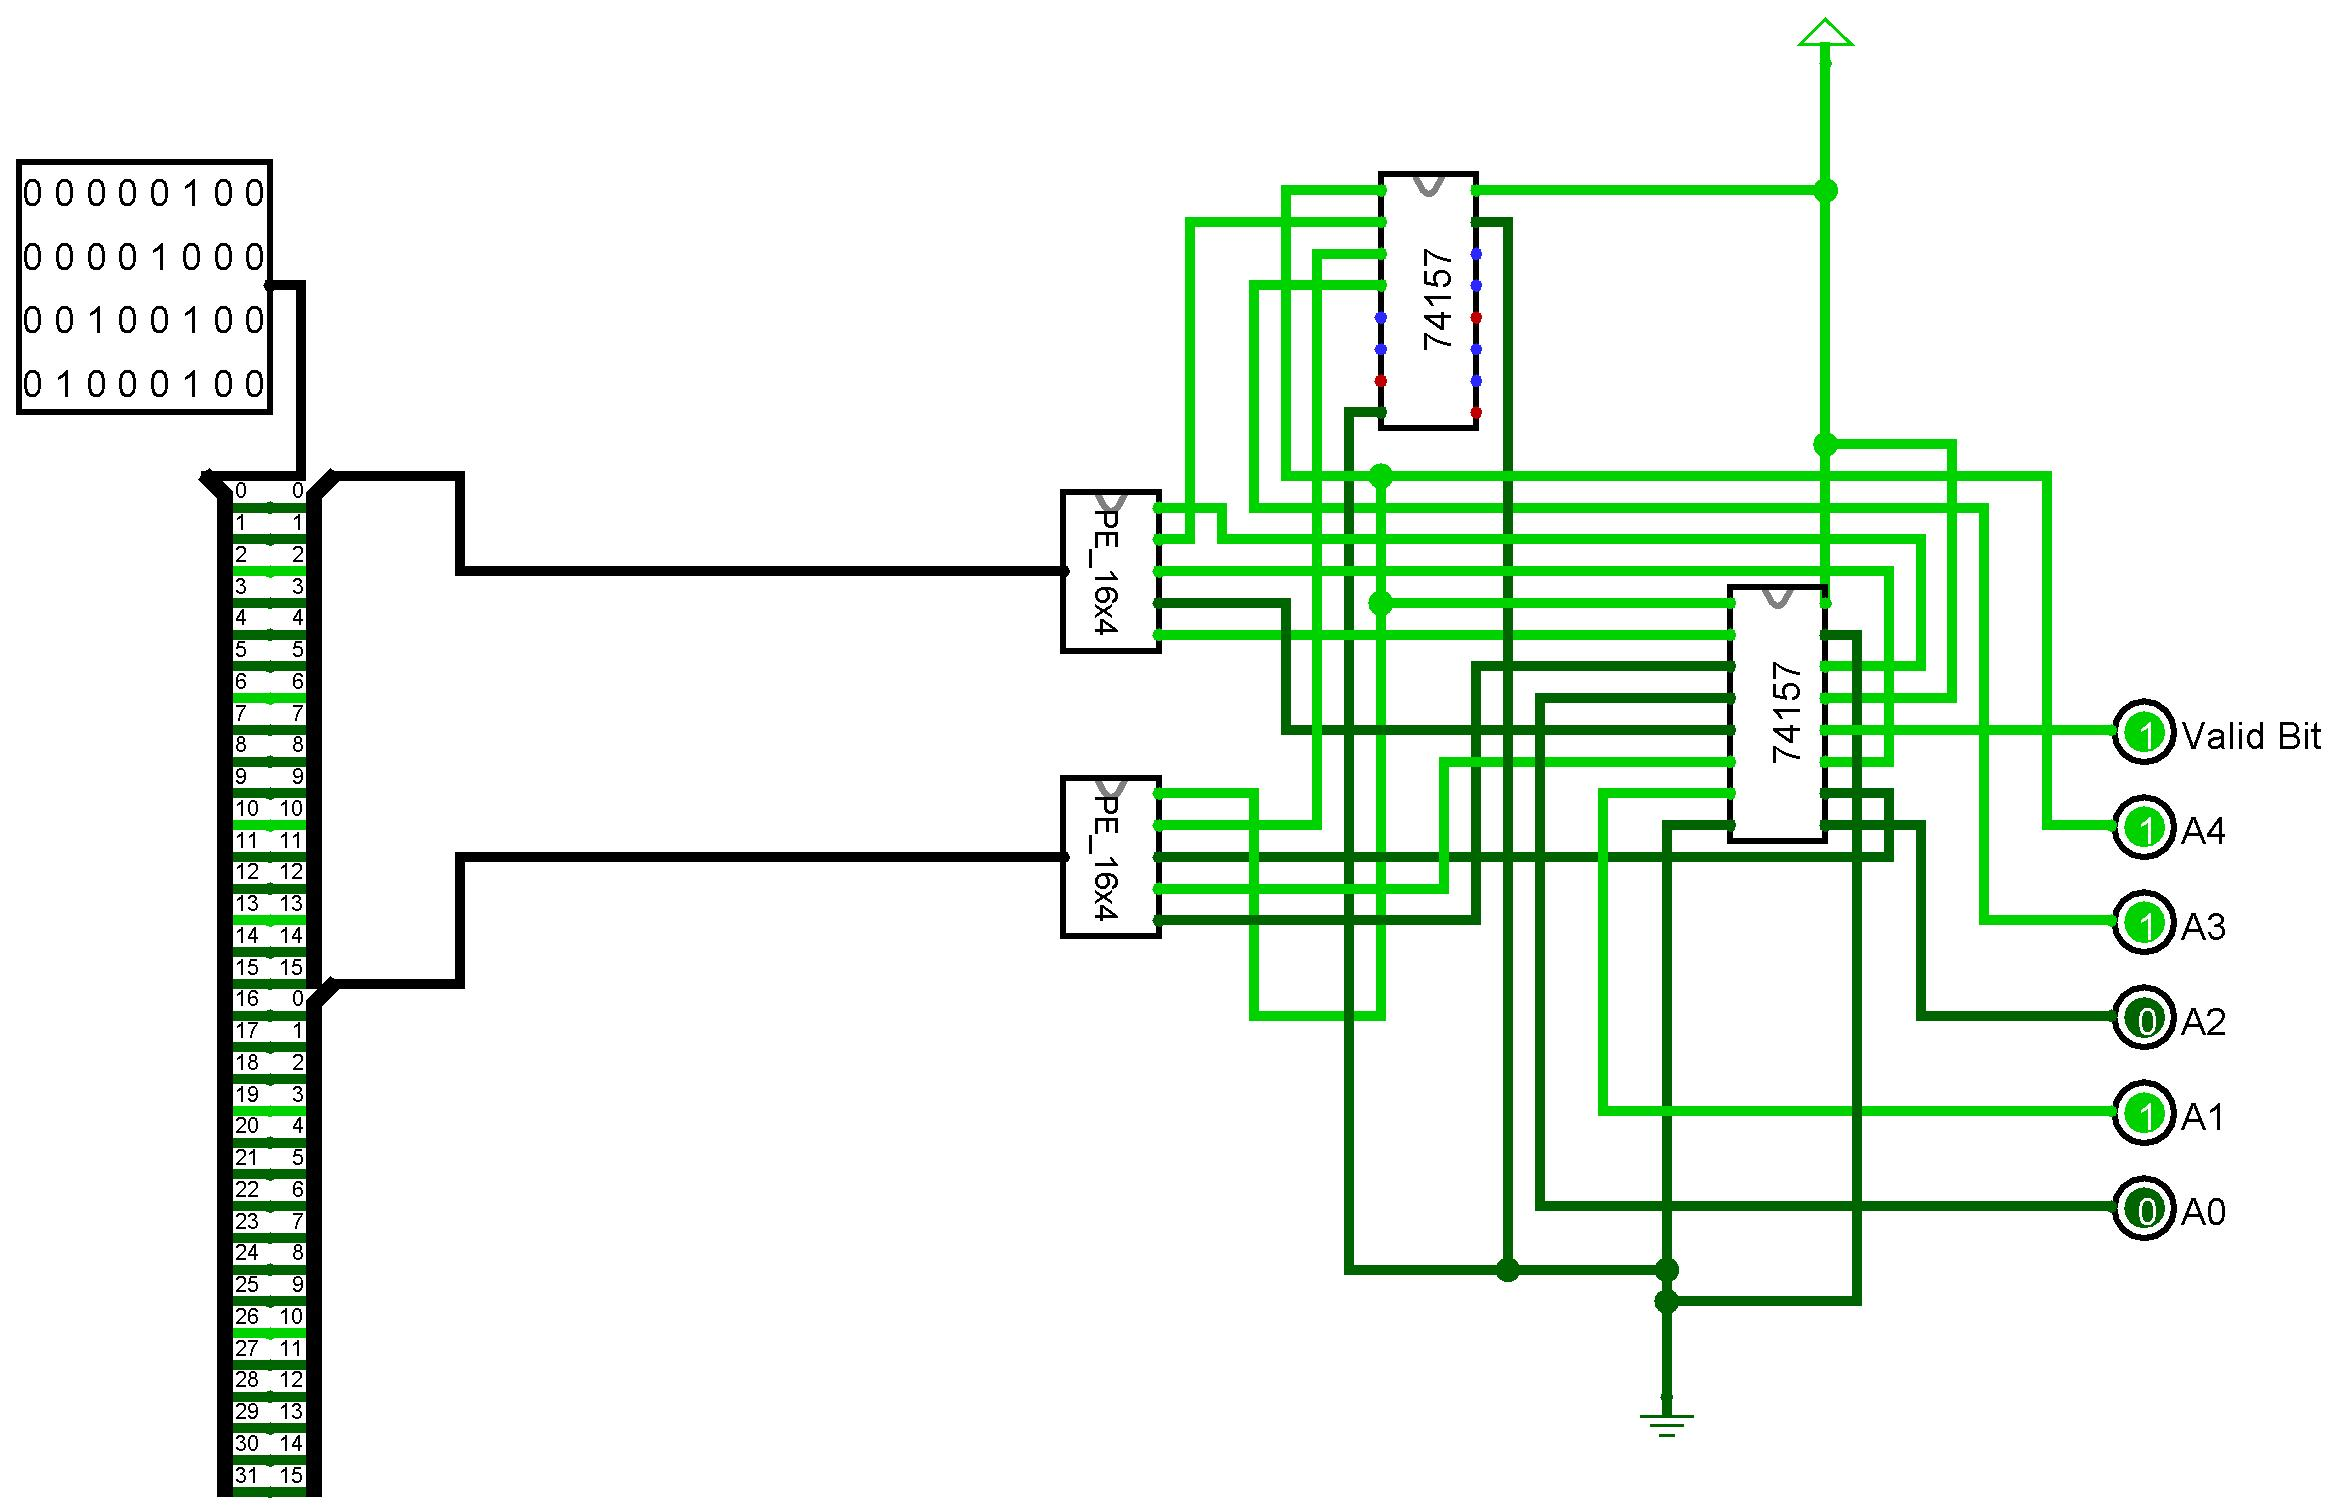
\includegraphics[width=\textwidth]{images/PE_32x5.jpg}
        \caption{32$\times$5 Priority Encoder}
        \label{fig:32x5prioenc}
    \end{subfigure}
    \caption{Encoder Circuits}\label{fig:encoder}
\end{figure}
\newpage
\subsection{Normalizer Circuit}
The normalizer circuit does necessary change in mantissa and exponent to change the number in operable form for other circuits.
\begin{figure}[H]
    \centering
        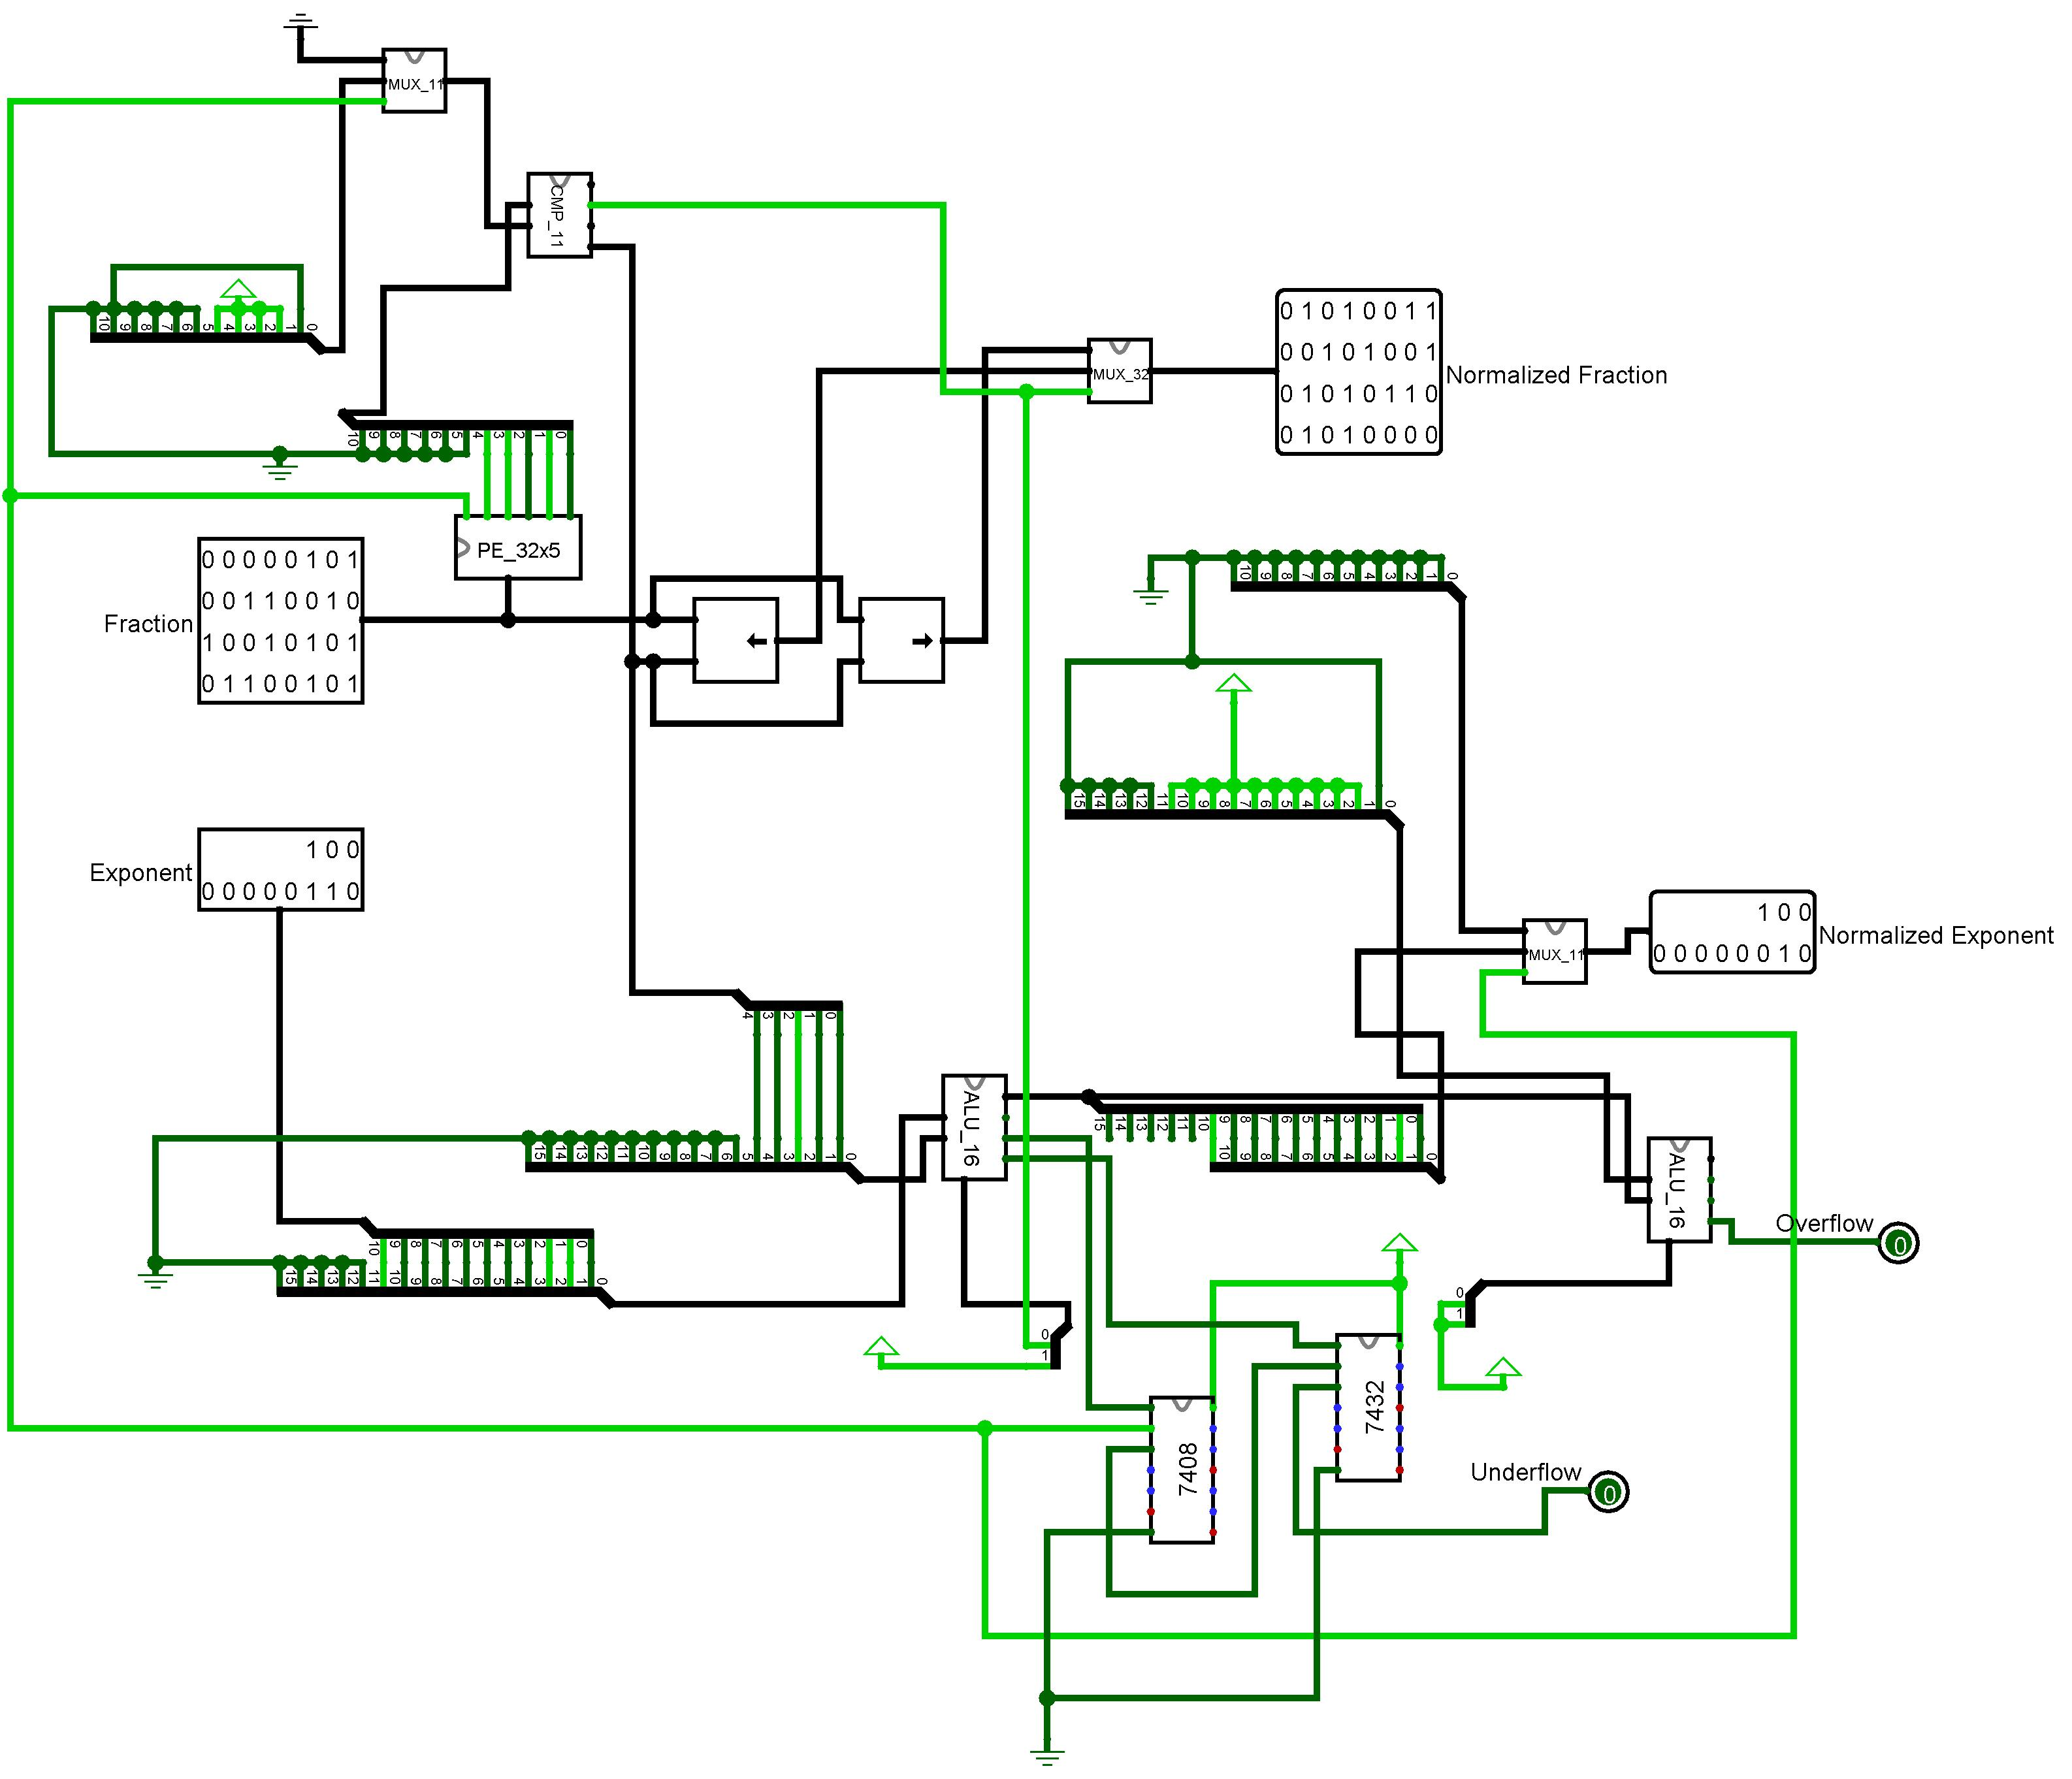
\includegraphics[width=\textwidth]{images/Normalizer.jpg}
    \caption{ Normalizer Circuit }\label{fig:normalizer}
\end{figure}


\newpage
\subsection{Rounder Circuit}
This circuit does the rounding of the mantissa in the result.
\begin{figure}[H]
    \centering
        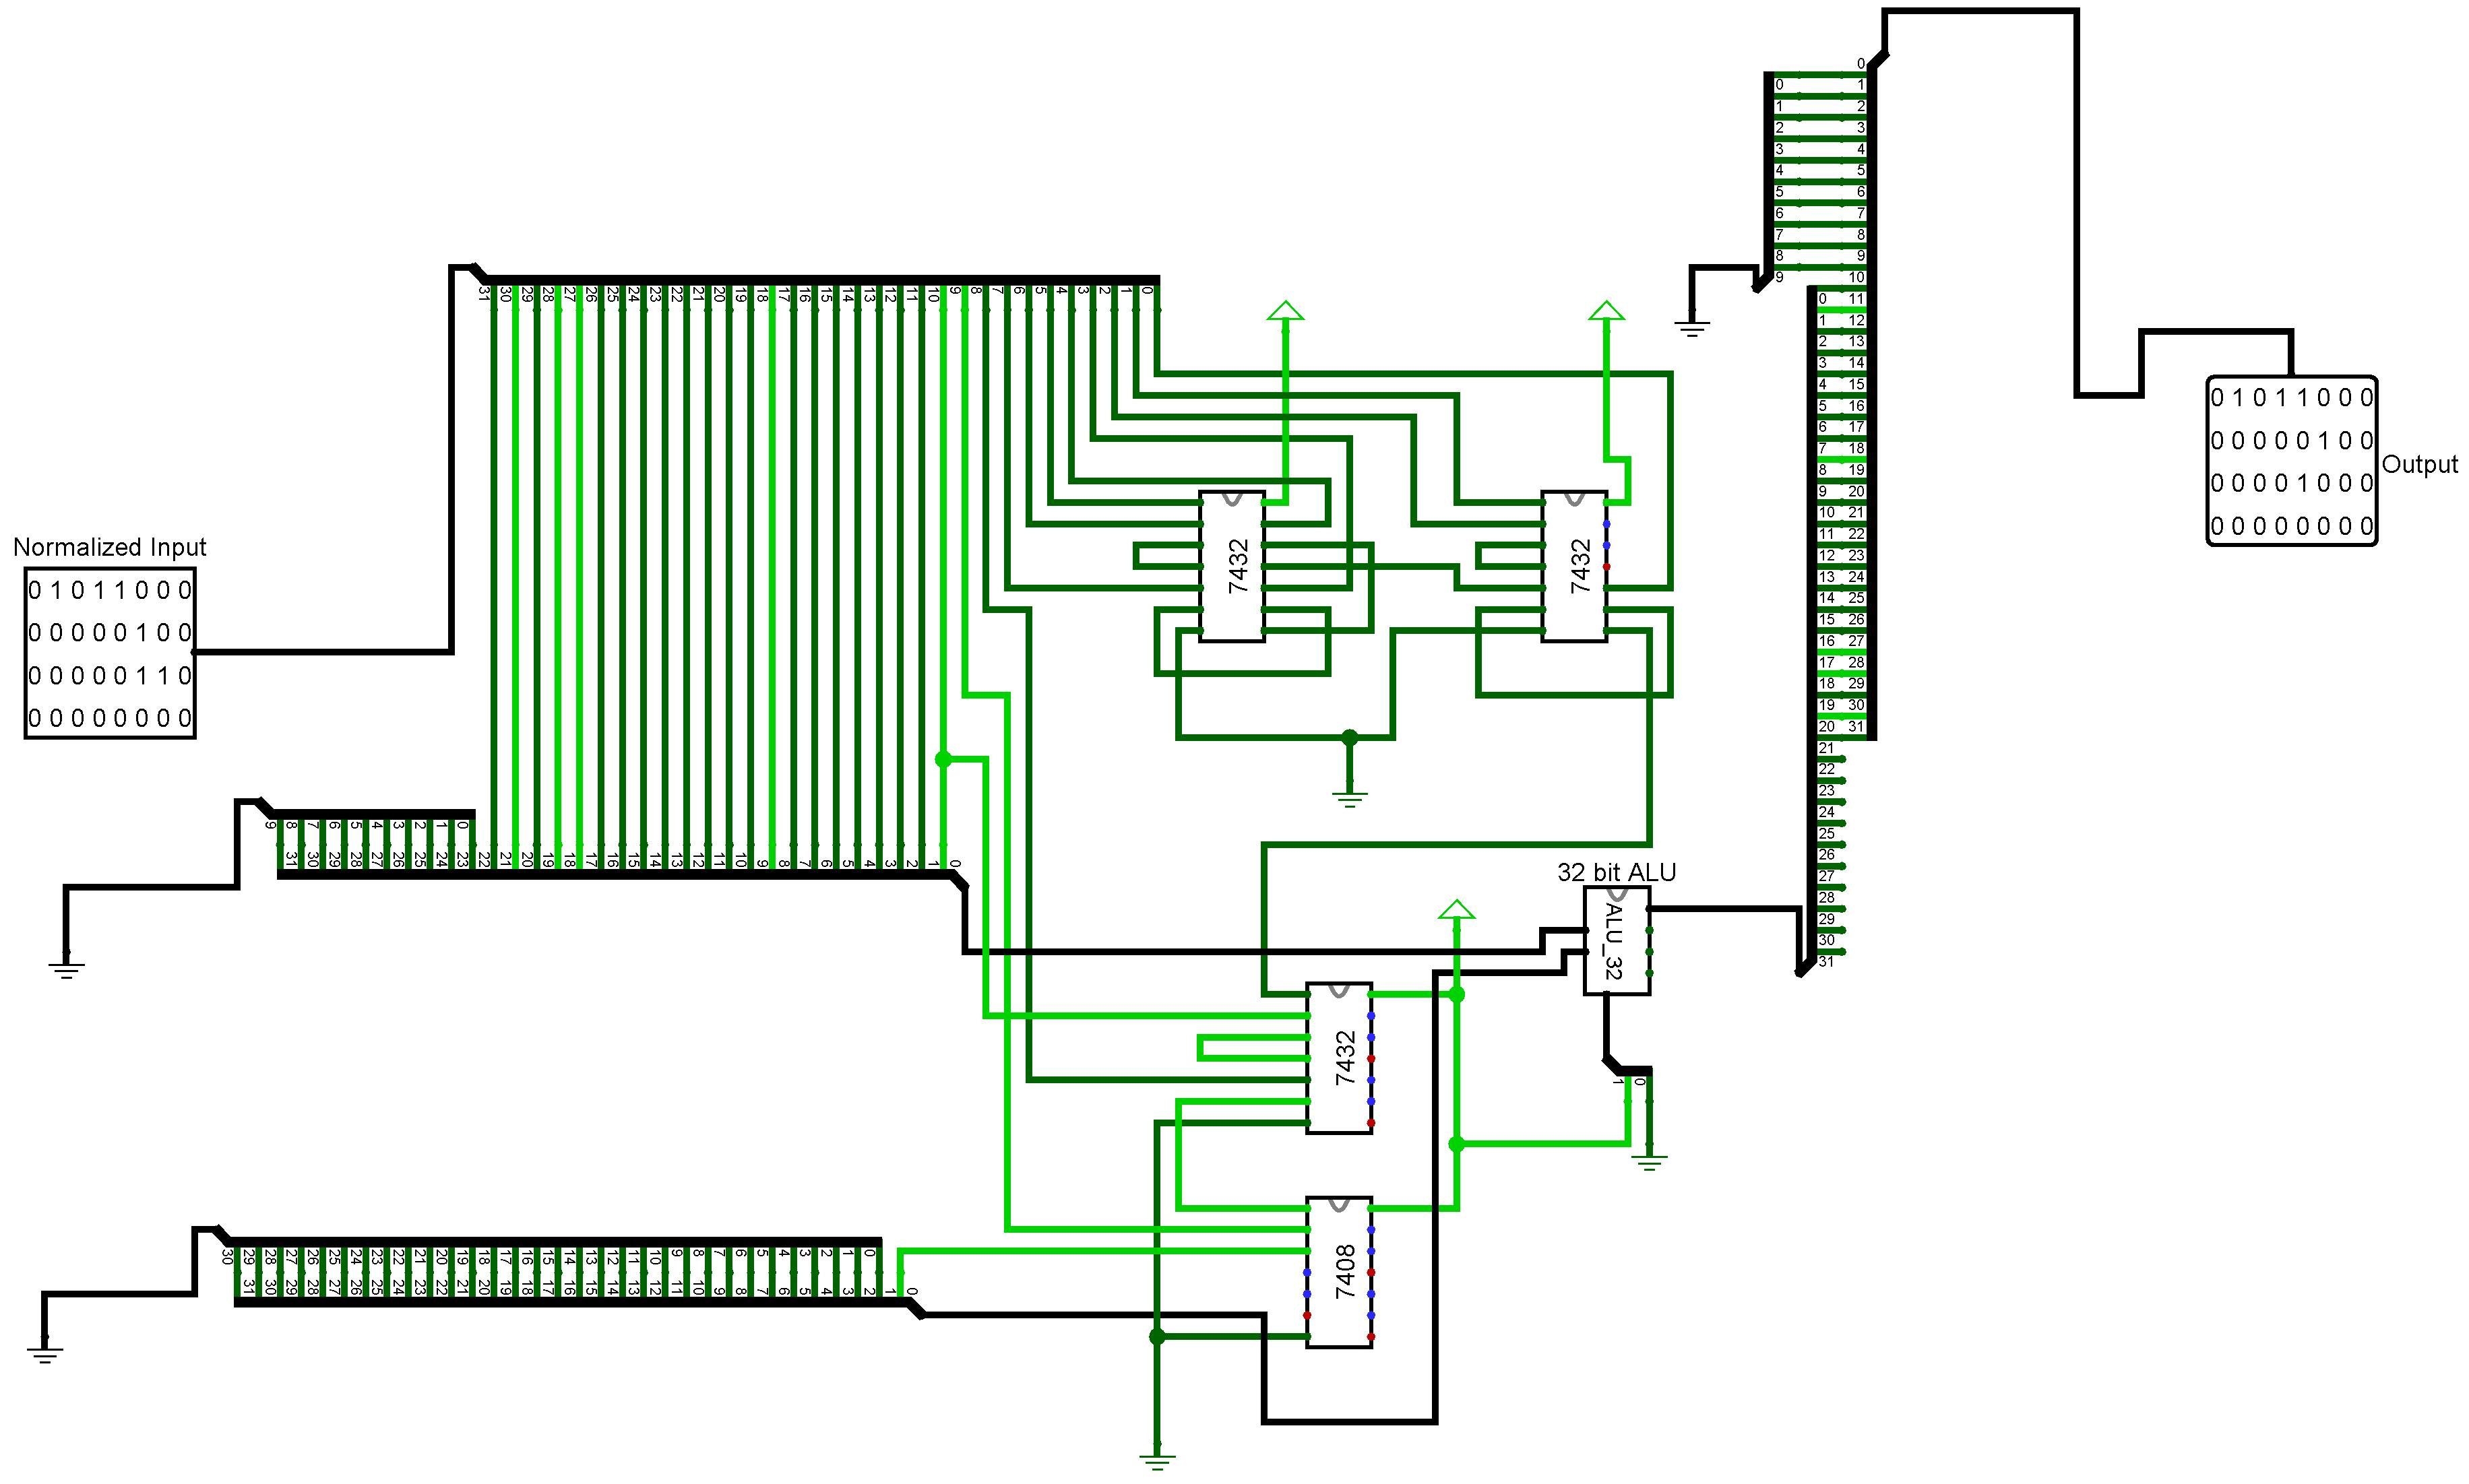
\includegraphics[width=\textwidth]{images/Rounder.jpg}
    \caption{Rounder}\label{fig:rounder}
\end{figure}

\vspace{2cm}

\subsection{Input Pre-processor Circuits}
This module validates the input given by user . It contains:
\begin{itemize}
    \item A Single Input Checker that shows the validity of a single floating point number input
    \item A Input Validator containing 2 single input checkers to validate the whole input
\end{itemize}
\begin{figure}[H]
\centering
  \begin{subfigure}[b]{\textwidth}
  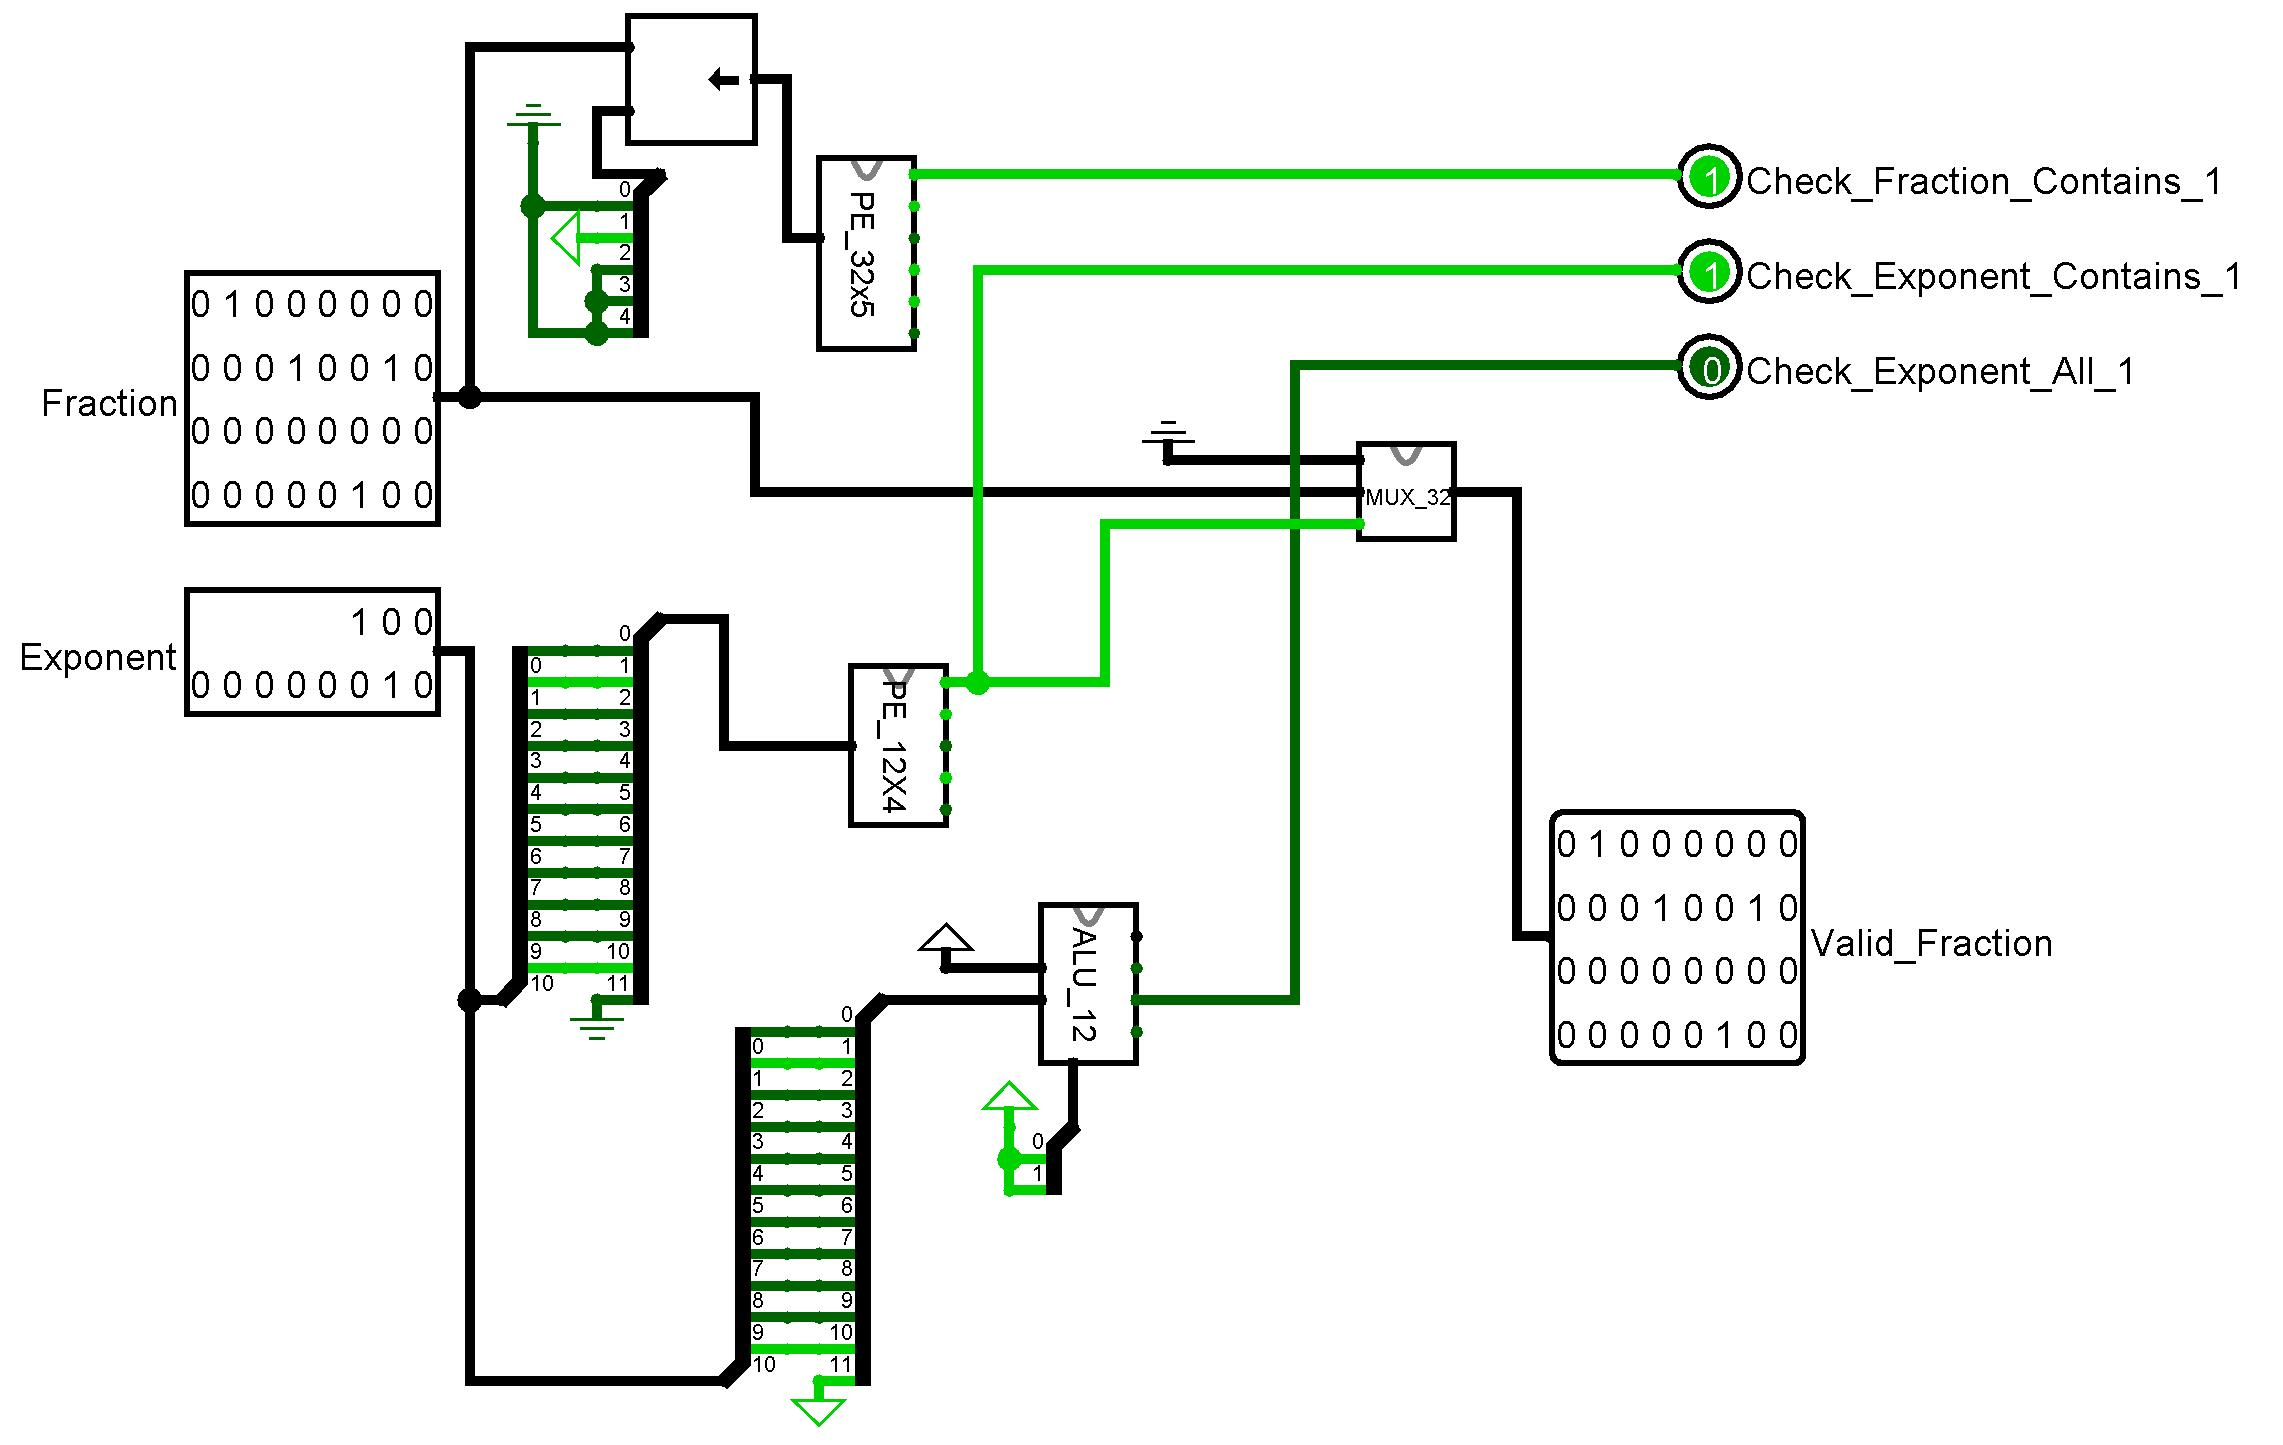
\includegraphics[width=\textwidth]{images/Single_Input_Checker.jpg}
  \caption{Single Input Checker}
  \label{fig:inpcheck}
  \end{subfigure}
  
 \begin{subfigure}[b]{\textwidth}
  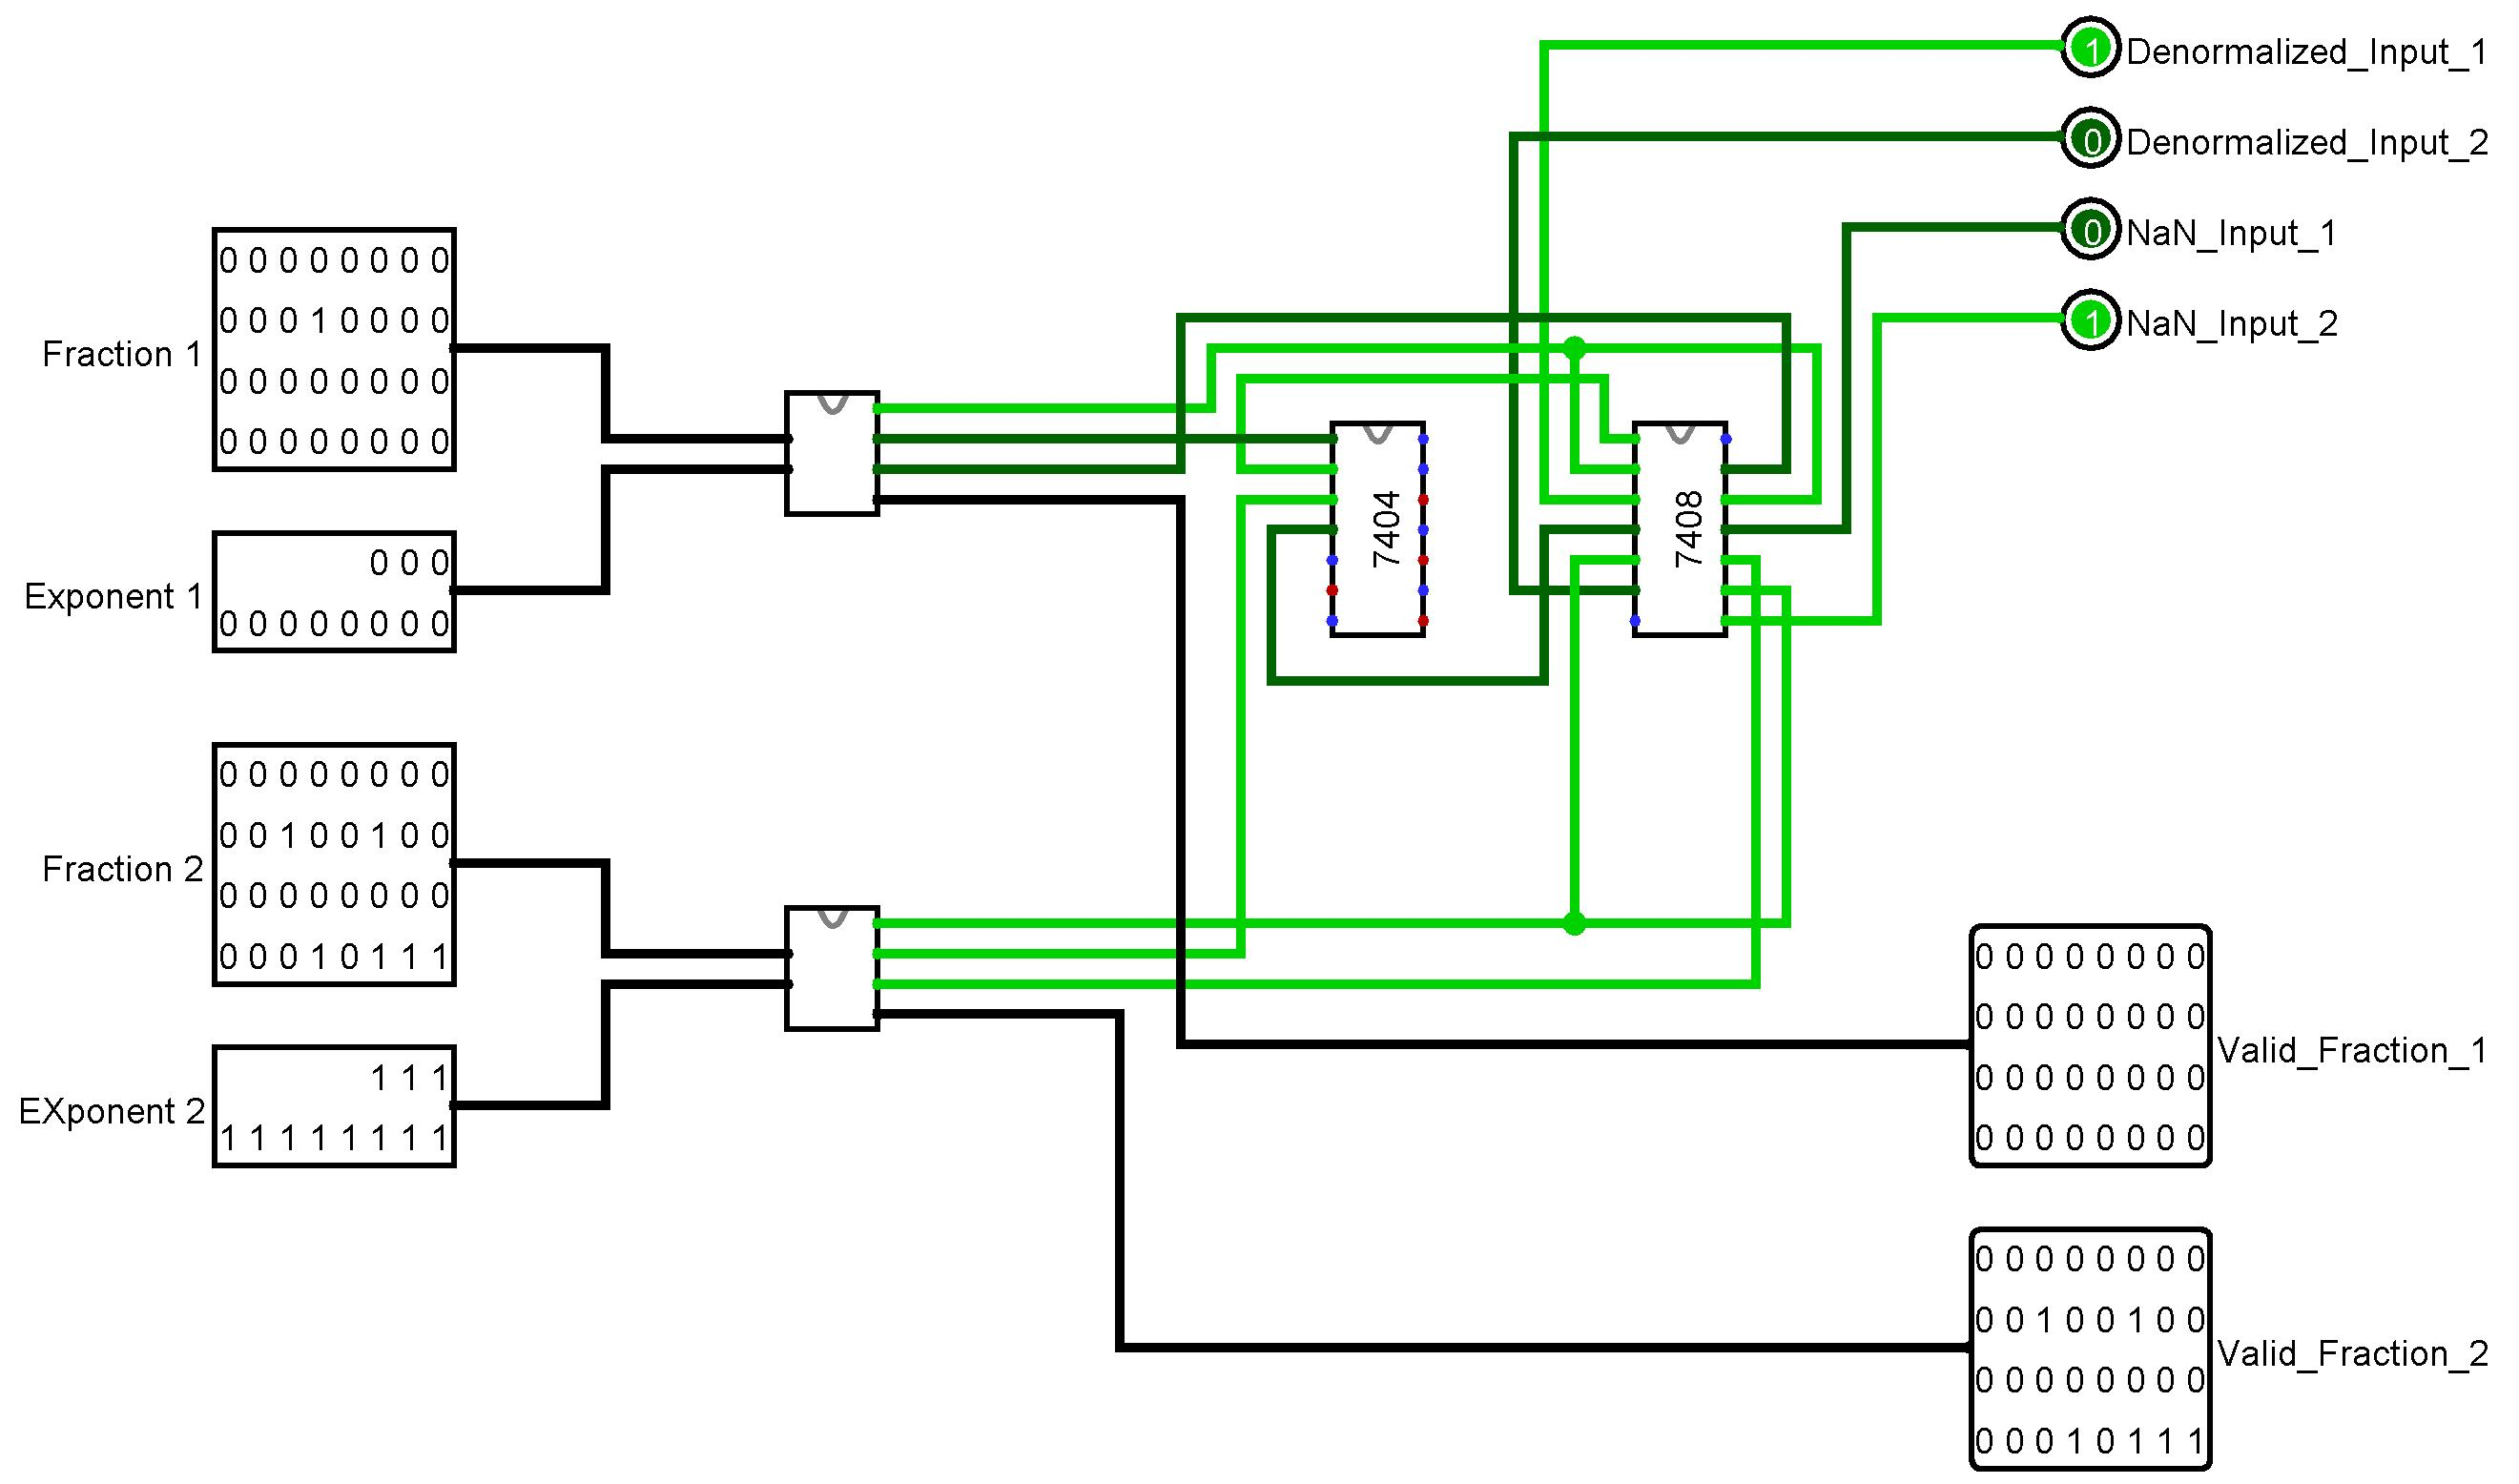
\includegraphics[width=\textwidth]{images/Input_Validator.jpg}
  \caption{Input Validator}
  \label{fig:inpval}
  \end{subfigure}
 \caption{Input Processing Utility}\label{fig:inpproc}
\end{figure}
\newpage
\subsection{Arithmetic Logic Unit}
The 32 bit Arithmetic Logic Unit is used in several places in the circuit to perform add operation. Additionally, 12 and 16 bit ALU's were also used in the design. All of them are of identical construct.
\begin{figure}[H]
    \centering
    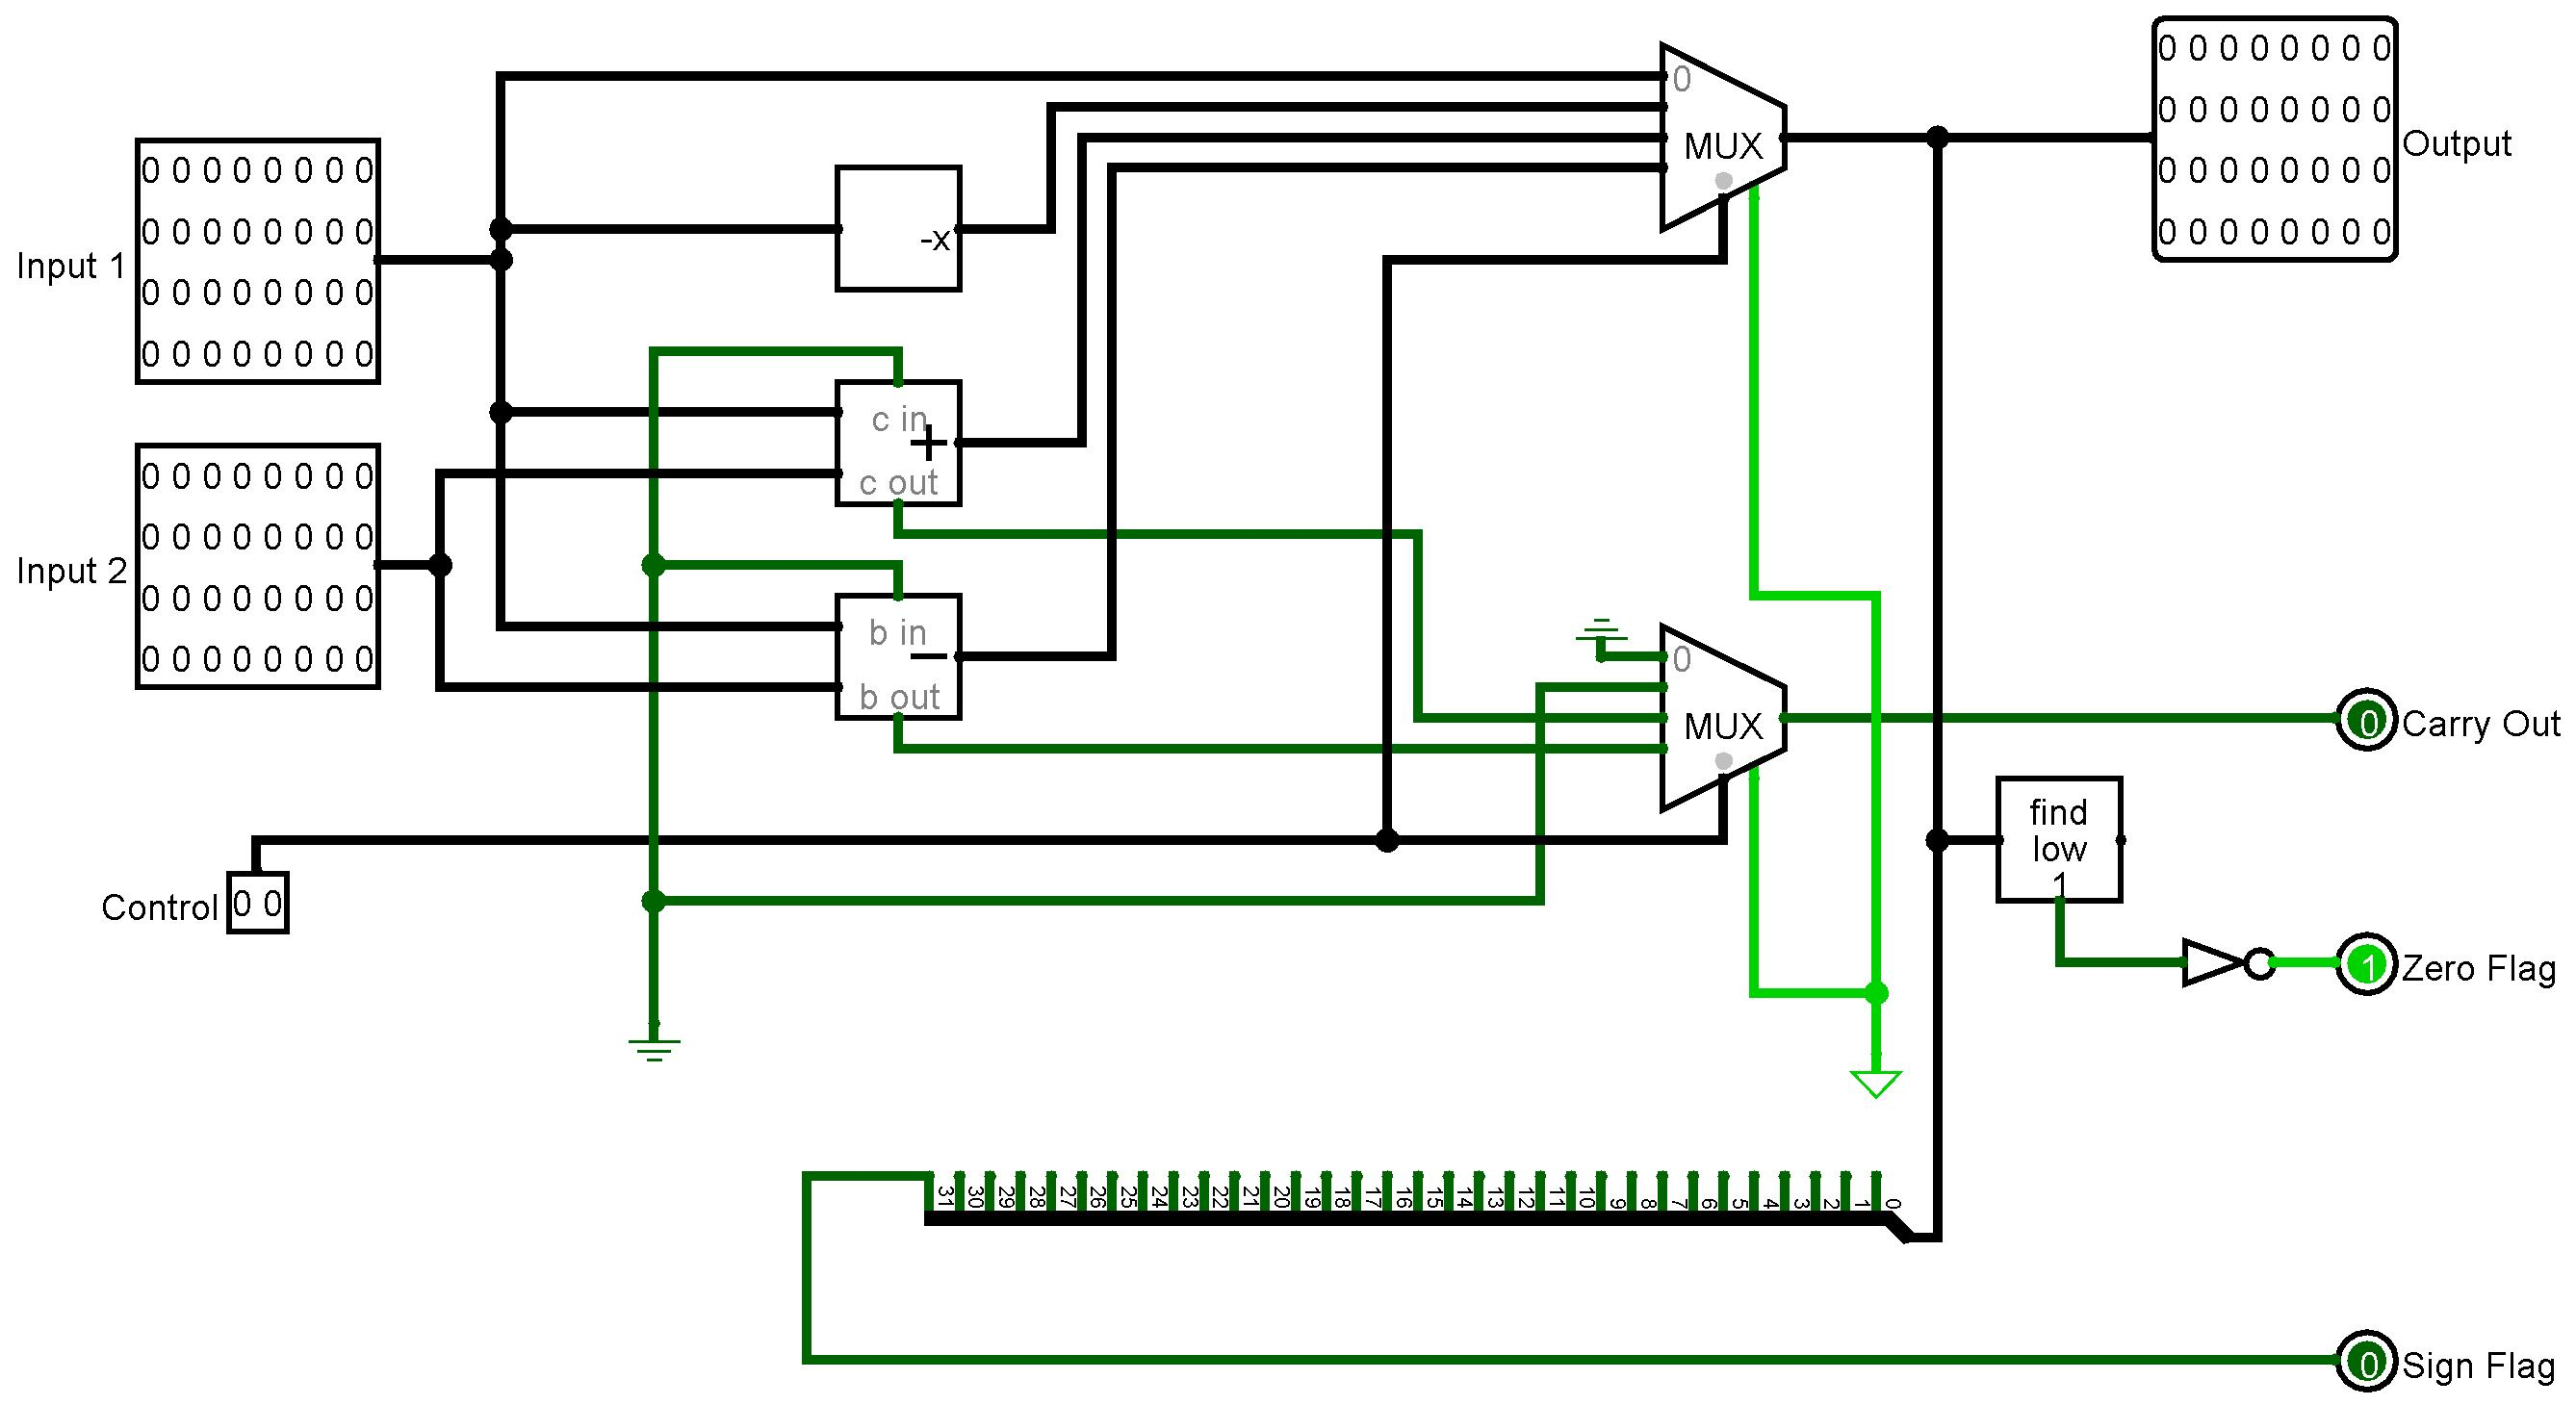
\includegraphics[width=0.7\textwidth]{images/ALU_32_bit.jpg}
    \caption{32 bit ALU}
    \label{fig:alu}
\end{figure}

\subsection{Floating Point Adder}
This is the actual floating point adder circuit which includes all the other libraries and circuits.
\begin{figure}[H]
    \centering
        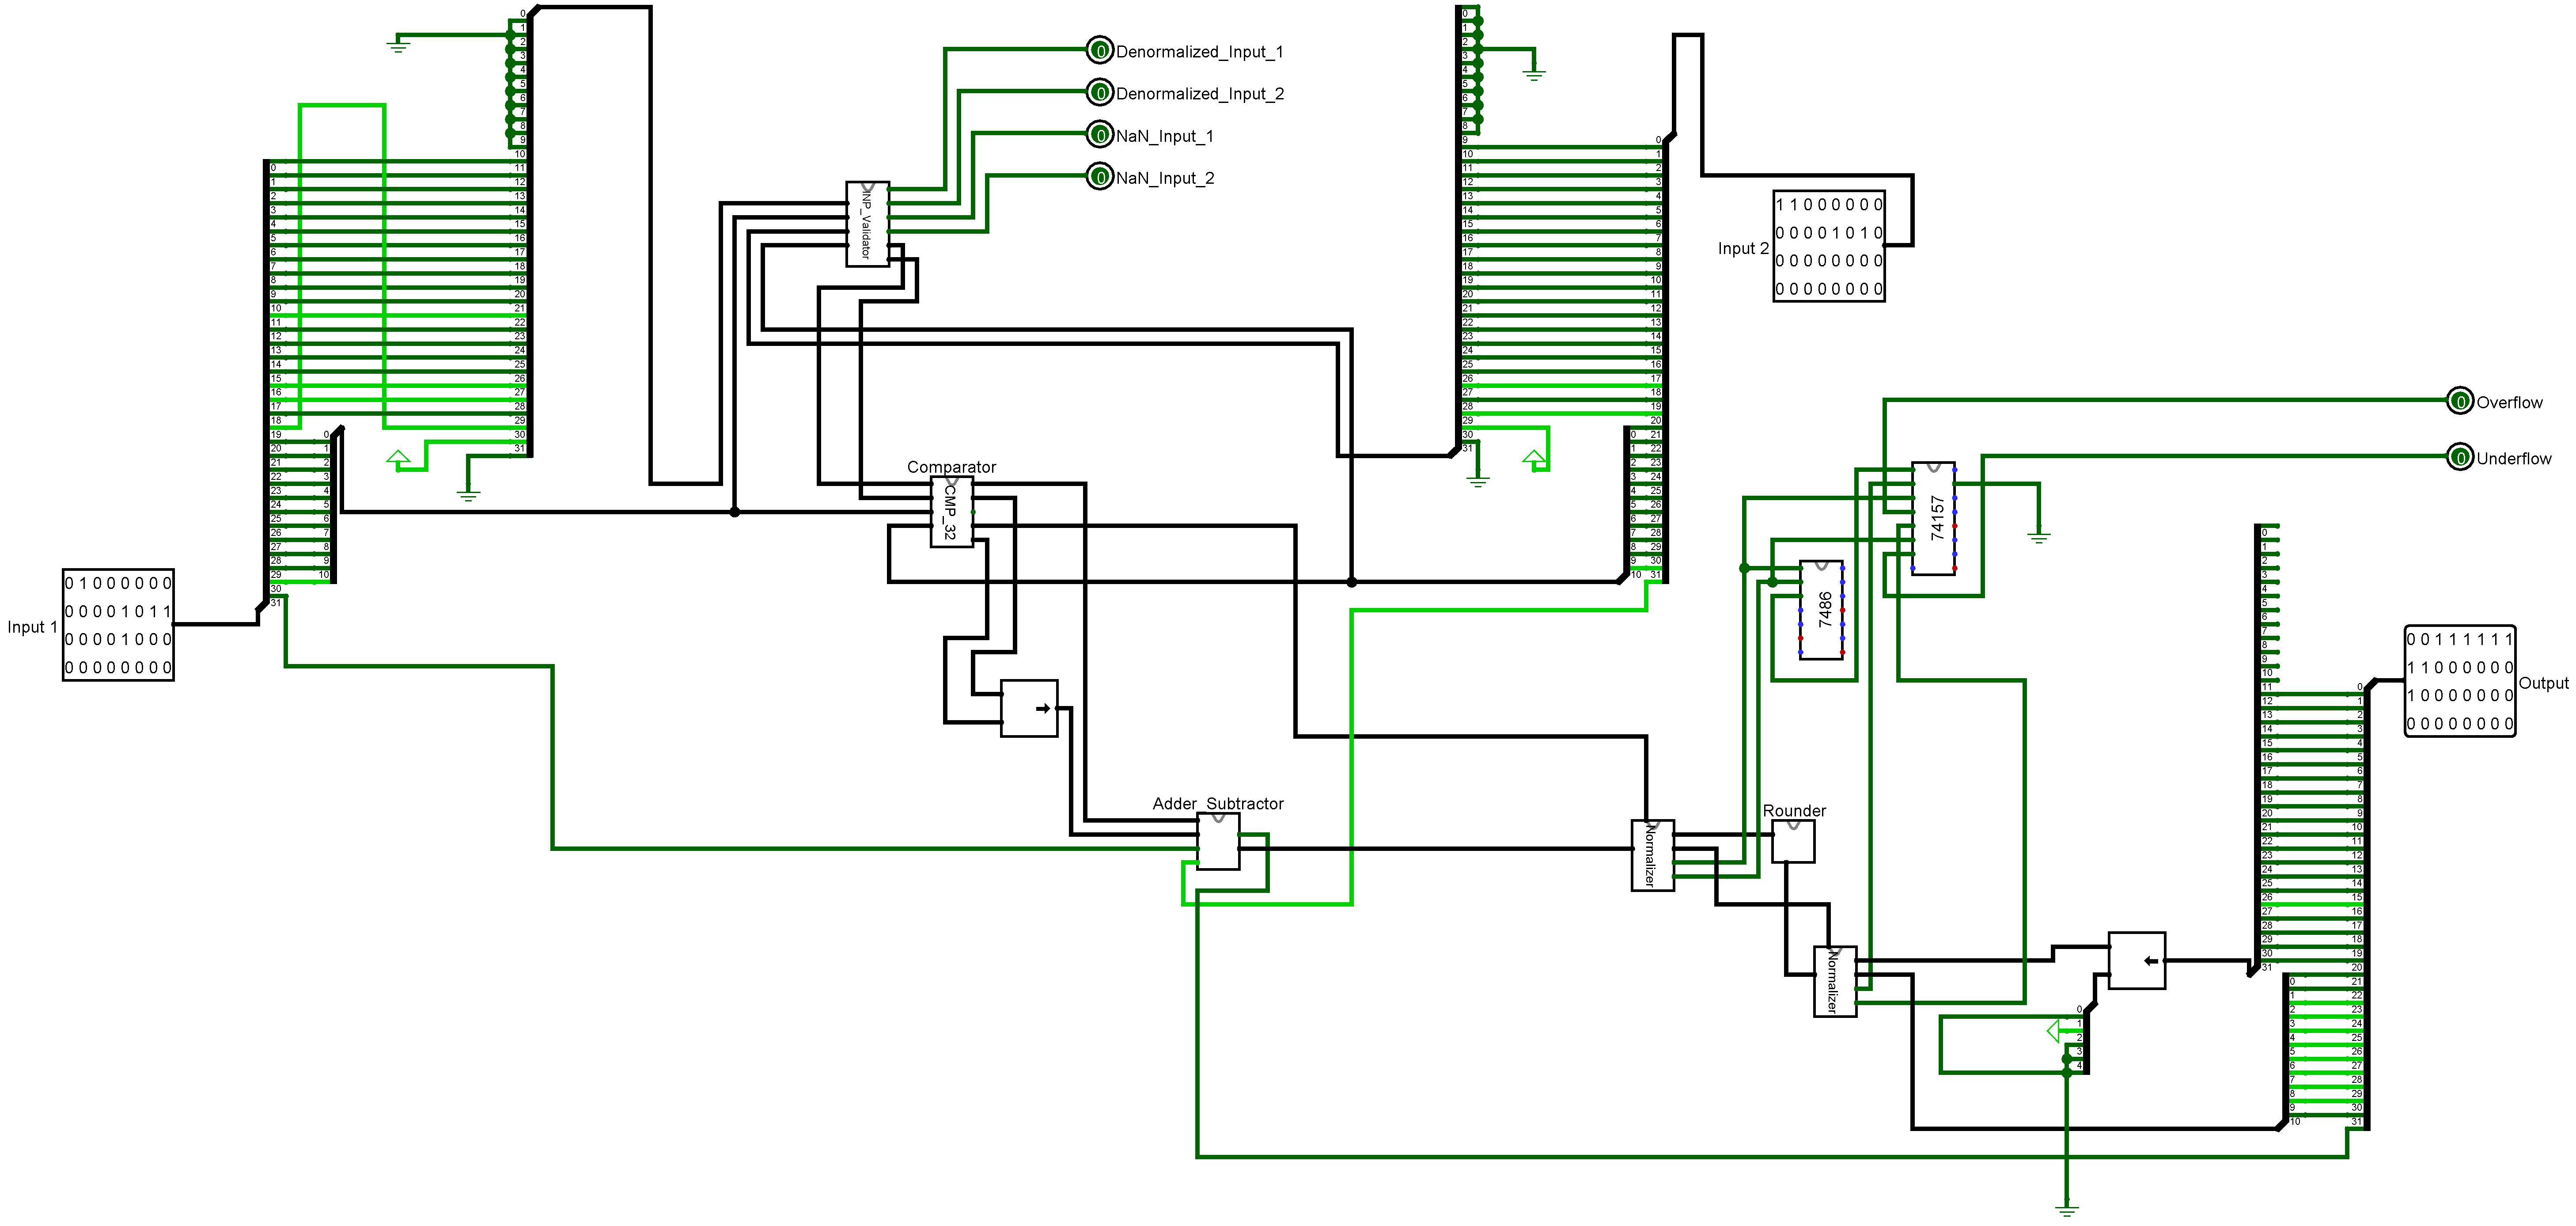
\includegraphics[width=\textwidth]{images/FPA.jpg}
    \caption{Floating Point Adder}\label{fig:fpa}
\end{figure}
\newpage
\subsection{Miscellaneous}
This is a circuit tester used for checking whether the output matches the desired answer or not. Using a RAM provided by the simulator software, the circuit checks our output against pre-generated outputs. It is a sequential circuit which increments the memory address by a counter at every clock pulse and matches output. 
\vspace{1cm}
\begin{figure}[H]
    \centering
        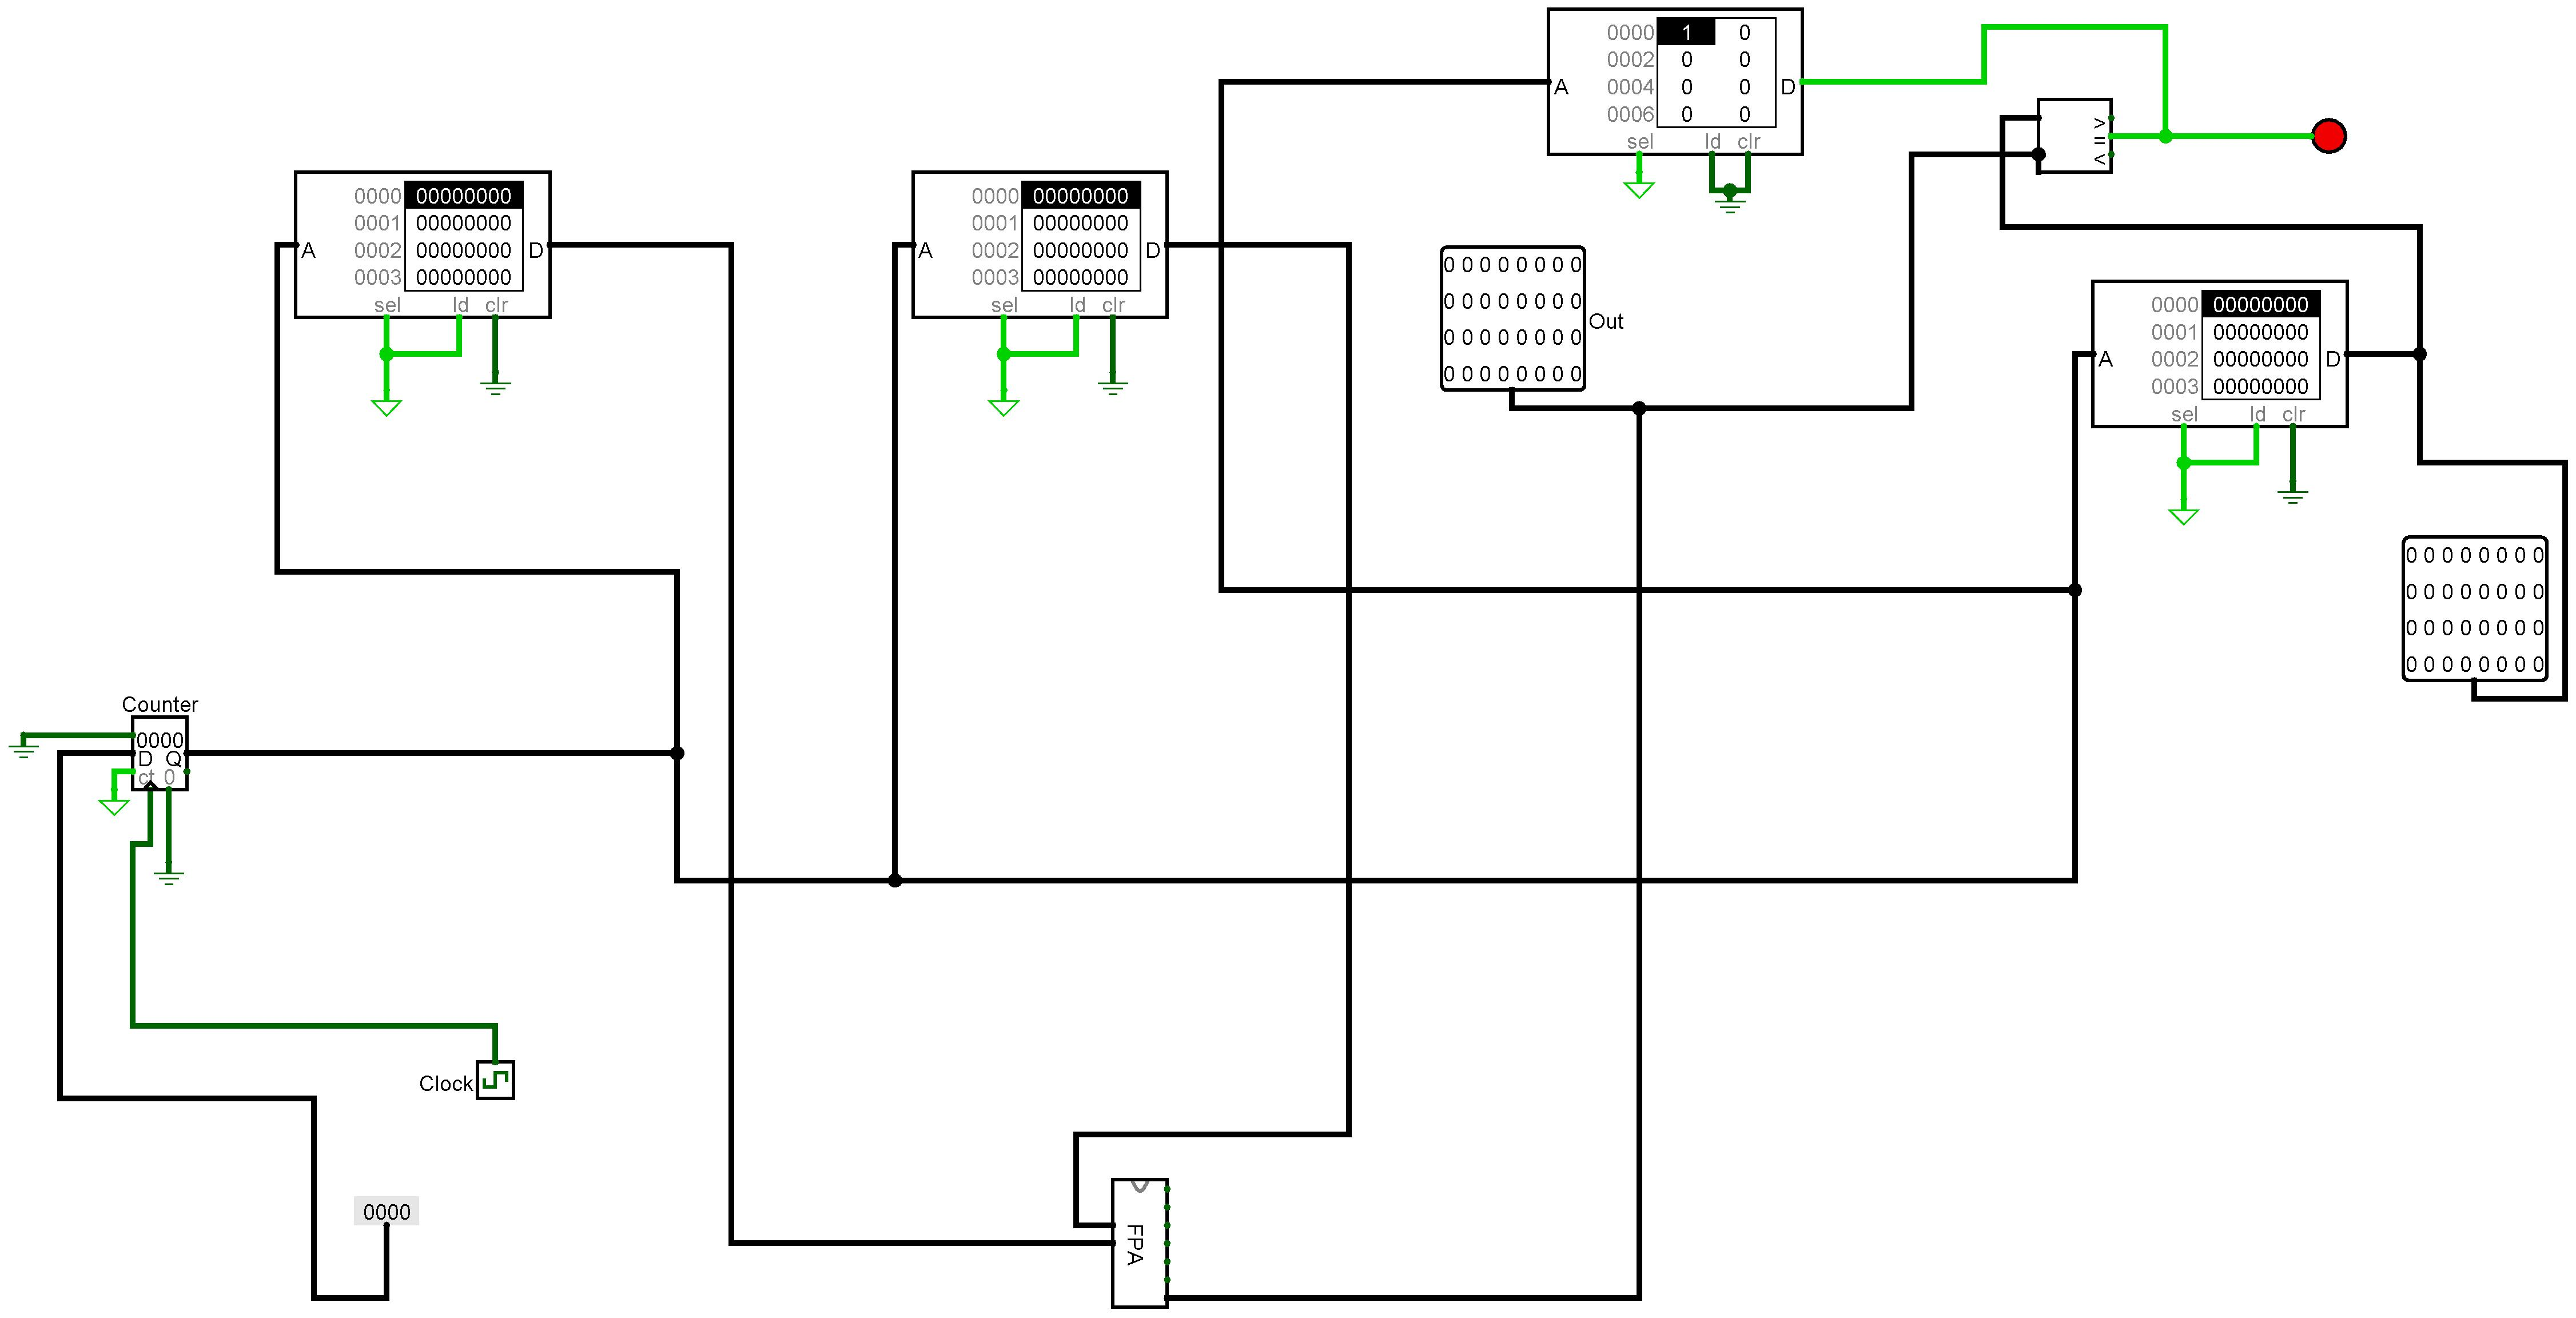
\includegraphics[width=\textwidth]{images/Circuit_Tester_Using_RAM.jpg}
    \caption{Circuit Tester}\label{fig:circtest}
\end{figure}




\newpage


% Section G - Jaber



\section{\large{ICs Used with Count as a Chart}}

\begin{table}[!h]
	\centering
	\begin{tabular}{|c|c|}
		\hline
		\textbf{IC} & \textbf{Quantity}  \\
		\hline
		IC 7404 & 2 \\
		IC 7408 & 5 \\
		IC 7432 & 6 \\
		IC 7486 & 2 \\
		IC 74148 & 20 \\
		IC 74157 & 123 \\
		ALU (12 bit) & 11 \\
		ALU (16 bit) & 4 \\
		ALU (32 bit) & 3 \\
		Shifter (Left) & 5 \\
		Shifter (Right) & 3 \\
		\hline
		Total & 184  \\
		\hline
	\end{tabular}
	\caption{ICs Used with Quantity}
	\label{tab:ic_quantity}
\end{table}

\newpage

\vspace{1cm}
\section{The Simulator Used along with the Version Number}
Logisim - 2.7.1


\newpage


\section{\large{Discussion}}

This assignment familiarizes us with a crucial aspect of Computer Arithmetic, named ‘Floating Point Addition’ in the light of IEEE 754 standard, a widely adopted floating-point formatting standard in modern computer systems.

\vspace{3mm}

First comes the process of building helping libraries containing circuits of similar genre and varying bit capacity. As of Encoder and Multiplexer libraries we used an ample amount of cascading to get to an understandable and maintainable design. The ALU library consisting of 3 different circuits, was built using default ‘Adder’ tools provided by the simulation software, as per the given specification. Comparator library saliently relies upon the ALU library for performing subtraction. Afterwards, it processes the output of the ALU to deliver information regarding comparison. 

\vspace{3mm} 

Next comes the major building blocks of the Floating Point Adder, Adder Subtractor, Input Validator, Normalizer and Rounder which are in turn built upon the aforementioned libraries. While designing these, we put utmost attention to minimizing the number of ICs by carefully altering myriad design decisions. For instance, previously we lacked the prospect of doing transfer operation in the ALU. Though it may seem unnecessary, in essence, it was costing us several extra Multiplexers. Upon realizing the same, we introduced the transfer operation in ALU. In the input validator, we implemented an error pre-checking mechanism, which, primarily with the help of Encoders and ALU, detects what IEEE specified range the inputs fall between. Accordingly, we showed output flags for whether the input is a ‘Denormalized Number’ or ‘NaN’ or valid. As for Rounder, omitting the appended ‘01’ in front, we considered 20 bits as actual mantissa, the two after them as ‘Guard’ and ‘Round’ bits, and all after them as Sticky bits. 

\vspace{3mm}

Designing the final circuit required merging the pre-built components while carefully handling the control flow. We performed Normalization again after Rounding, since, in an extreme case, the output from the Normalizer may turn out to be denormalized after being processed by the Rounder. Overflow, Underflow and Error checker flags were shown as outputs in the final circuit. As we appended two bits ‘01’ in front of the mantissa to imitate the hidden set bit, while showing the output, we had to ignore those two bits using a left shifter. 

\vspace{3mm}

To verify our outputs, we wrote a python script to generate bulk random inputs and corresponding outputs. Afterwards, we used the provided RAM in the Logisim simulation software to build a sequential circuit driven by clock pulses. At every clock pulse, it enhances the address by 1, locates the next position, reads the data, performs the simulation and writes it back to another RAM. We then read back that RAM and match the outputs with our pre-calculated outputs. 

\vspace{3mm}

Since the design process incorporates a deep hierarchy of components, counting the total number of ICs required for the whole design was a challenging task to do by hand. Therefore, we first converted our design into a Directed Graph format, which indicated which components hold which other components as children at what count. We then wrote another python script to run a Depth First Search on the directed graph to count the number of ICs through bottom-up Dynamic Programming. 

\newpage

\vspace{3mm}

While building through, at numerous junctions, we had to choose among several different design decisions and we hope we managed to take the optimal path in most of those cases. Extensive randomized and automated testing was performed afterwards, which further enkindles the hope that ours has been a fully working optimized design. 

\vspace{3mm}

We wish to learn a lot more about the miniscule details of the design and we hope to extend our design to incorporate further operations in future.


\end{document}
